% !TeX program = pdflatex
\documentclass[preprint,12pt]{elsarticle}
\journal{Computer Networks}
\usepackage{amsmath,amssymb,amsthm,booktabs,graphicx,algorithm,algorithmic,multirow}
\usepackage{float}
\newtheorem{proposition}{Proposition}
\emergencystretch=1.5em
\usepackage{tikz}
\usetikzlibrary{arrows.meta,positioning,fit,calc}

\begin{document}
\begin{frontmatter}
\title{FedRAS: Network-Conditioned Rank Allocation for Federated LoRA}
\author[inst1,inst2,inst3]{Wenyu Ma}
\author[inst1,inst2,inst3]{Tao Hu\corref{cor1}}
\author[inst1,inst2,inst3]{Xinlei Liu}
\cortext[cor1]{Corresponding author}
\ead{hutaondsc@163.com}
\address[inst1]{Information Engineering University, Zhengzhou 450001, China}
\address[inst2]{Key Laboratory of Cyberspace Endogenous Safety and Security of Henan Province, Zhengzhou 450001, China}
\address[inst3]{Key Laboratory of Cyberspace Security, Ministry of Education of China, Zhengzhou 450001, China}

\begin{abstract}
Federated LoRA reduces update size, but a fixed rank cannot adapt to time-varying links. We formulate rank selection and client admission as a joint network scheduling problem and call the resulting method FedRAS. It estimates delivery probability and adaptation capacity for each client--rank pair, maximizes expected useful updates under budget and participation constraints, solves the assignment by dynamic programming, and aggregates heterogeneous ranks with frozen-factor rank masking.

Trace-driven experiments couple a real federated LoRA trainer on non-IID CIFAR-10, CIFAR-100, and MNIST with a 500-client scheduling simulator, external baselines, ablations, and sensitivity analyses. Under nominal deadlines every rank preserves backbone accuracy while full-parameter updates spend $2.2\times$ the bytes for no gain. Under deadline stress FedRAS downshifts to delivered rank 13.5, matches fixed rank 16, and saves 14\% of bytes in the reported ten-seed comparison at $p{=}0.002$. Full-parameter updates miss 96\% of deadlines in the same setting, while the simulator reports 73\% fewer timely updates than rank-16 LoRA. The dynamic program is exact for the discretized single-round estimated assignment problem and improves on greedy scheduling by up to 10\% in binding regimes at 33--836\,ms solver cost. These results describe network-side gains in the evaluated frozen-CNN setting and do not imply universal accuracy gains.
\end{abstract}

\begin{keyword}
Federated LoRA \sep Mobile edge computing \sep Rank selection \sep Deadline scheduling \sep Wireless federated learning
\end{keyword}
\end{frontmatter}

\section{Introduction}
\label{sec:intro}

Mobile edge networks increasingly host federated learning (FL) workloads in which heterogeneous clients such as smartphones, vehicles, UAV terminals, and satellite-connected devices collaborate on a shared model without exposing raw data \cite{mcmahan2017fedavg,kairouz2021advances,liu2018sagin,mahboob2024ntn}. The dominant cost in such systems is the uplink. Full-parameter model updates saturate wireless capacity, drain client energy, and frequently miss round deadlines when links degrade during handover or outage, as reported for ground, aerial, and satellite segments \cite{razmi2022ground,tang2023flsagin,qin2024dfrl,ribero2023intermittent}. Low-rank adaptation (LoRA) has therefore become an attractive transmission format for FL, because only two small factor matrices per adapted layer are communicated instead of the full weight delta \cite{hu2022lora,babakniya2023slora,zhang2024fedit}.

Existing Federated LoRA systems, however, treat the rank $r$ as a model hyperparameter. The rank is selected from data and system constraints alone, possibly varying across clients \cite{cho2024hetlora,fan2025helora} or adapting across rounds \cite{wu2026fedara,yang2024safedlora}, but not from the state of a lossy, deadline-constrained link. This convention ignores a scheduling dimension that is directly visible to the network. The rank determines the number of transmitted parameters and hence the transmission time. On a time-varying link, a larger rank raises the probability that the update misses the round deadline $\tau$, while a conservative small rank underuses a stable link and limits how much adaptation each round can carry. Thus, rank is also a network scheduling variable. Per-client, per-round rank selection converts link heterogeneity into a trade-off between adaptation capacity and timely delivery.

This raises three questions. How should delivery probability depend on rank and observable link state? How should client--rank assignment be solved under budget and participation constraints? Does the resulting adaptation improve network behavior in a real trainer?

\subsection{Contributions}
We answer these questions with a delivery model, a grid-based dynamic-programming solver, a rank-selection rule, and a two-tier evaluation. We call the method FedRAS. The contributions are as follows.

\begin{itemize}
\item \textbf{Deadline-aware client--rank model.} We formulate each round as a joint assignment in which admission and rank are selected together. The model links rank to payload, delivery probability $P_{\mathrm{on}}(r)$, and saturating capacity gain $G(r)$. Sections~\ref{sec:model} and \ref{sec:problem} develop the model.
\item \textbf{Dynamic-programming scheduler.} The estimated problem is a multiple-choice knapsack with an admission cap. We derive a pseudo-polynomial dynamic program that is exact for the discretized single-round estimated assignment problem, with complexity $O(|\mathcal D| K B_{\max}|\mathcal R|)$. The solver study measures greedy gaps and runtime.
\item \textbf{Heterogeneous-rank aggregation.} We use rank-masked averaging with a shared frozen $A$ factor. Under this condition, the rule gives exact coordinate-wise averaging of active induced-update slices and avoids dilution of high-rank coordinates. Proposition~\ref{prop:agg} states the conditions and limits.
\item \textbf{Two-tier evaluation.} A real trainer covers non-IID CIFAR-10, CIFAR-100, and MNIST. A 500-client simulator covers deadline, budget, mobility, and scale regimes. At 0.25\,s, FedRAS reaches mean delivered rank 13.5, has comparable accuracy and timely delivery to fixed rank 16, and saves 14\% of bytes. The evaluation also includes baselines, ablations, sensitivity studies, and a trainer comparison of full grid scheduling and fair-cohort scheduling.
\end{itemize}

A preliminary poster version of this work studied joint client--protection scheduling for federated learning in space--air--ground mobile networks \cite{ma2026mswim}. The present article substantially reformulates that line of work around a different schedulable resource. It replaces compression-and-protection policies with the LoRA rank as the per-client decision variable. It introduces the MB-to-Mbit delivery hazard and the saturating capacity model of Section~\ref{sec:model}, replaces the heuristic admission-and-repair procedure with a dynamic program that is exact on the stated budget grid, and adds frozen-factor rank-masked aggregation for heterogeneous ranks. It also reports a new two-tier evaluation comprising a real federated LoRA trainer, a 500-client scheduling simulator, and a solver exactness study. Accordingly, all numerical results in this article come from the revised formulation and implementation and are not comparable with the preliminary version.

We report accuracy, timely delivery ratio, and bytes per round separately. With a frozen pretrained backbone, the expected benefit of rank selection is on the network side rather than universal accuracy improvement.

The remainder of this paper is organized as follows. Section~\ref{sec:related} reviews related work. Section~\ref{sec:model} introduces the system model. Section~\ref{sec:problem} formulates the scheduling problem and Section~\ref{sec:solver} presents the solver and the aggregation scheme. Section~\ref{sec:eval} reports the evaluation, Section~\ref{sec:discussion} discusses limitations, and Section~\ref{sec:conclusion} concludes.

\section{Related work}
\label{sec:related}

\subsection{Parameter-efficient and federated LoRA}
LoRA freezes a pretrained backbone and learns low-rank increments $\Delta W=BA$ \cite{hu2022lora}. Federated LoRA trains these adapters across clients. Prior work has studied sparse updates, instruction tuning, and model-heterogeneous personalization \cite{babakniya2023slora,zhang2024fedit,yi2026pfedlora}. A further line lets the rank vary across clients and aligns the results for aggregation, by rank self-pruning with sparsity-weighted averaging \cite{cho2024hetlora}, stacking \cite{wang2024flora}, zero-padded rank alignment \cite{fan2025helora}, or SVD-based dynamic rank allocation \cite{wu2026fedara}.

FFA-LoRA \cite{sun2024ffalora} froze one factor at its random initialization and showed that this improves stability in privacy-preserving federated fine-tuning. We adopt the same frozen-factor property for a stronger reason. When the frozen factor is identical across clients, averaging the trainable factor gives exact coordinate-wise averaging of the active induced-update slices, as Proposition~\ref{prop:agg} shows. It thereby removes the factor-rotation inconsistency that we show empirically to destabilize joint A/B training. Section~\ref{sec:aggregation} develops this aggregation.

SA-FedLoRA schedules rank over rounds without conditioning on link state \cite{yang2024safedlora}. FedSA-LoRA studies asymmetric factor aggregation with client-local parameters \cite{guo2025fedsalora}. These rank-adaptation rules respond to training progress or device capability, not to the delivery state of a deadline-constrained link. We evaluate an annealing baseline and joint A/B averaging while making rank a per-round decision conditioned on delivery state and deadline.

\subsection{Communication-efficient federated learning}
A broad literature reduces FL communication through sparsification, quantization, compressed sensing, and over-the-air aggregation \cite{oh2023fedqcs,oh2024fedvqcs,liu2023adaptivequant,kim2023beamforming,reisizadeh2020fedpaq,lin2018deep}. These methods compress a given update. Our scheduler selects its rank before transmission, so rank directly affects payload and deadline feasibility. The proposed capacity and delivery models can therefore be combined with other codecs.

\subsection{Client selection and deadline-aware scheduling}
Client selection improves FL efficiency under data, latency, and energy heterogeneity \cite{oort2021oort,chen2024clientselection,dong2024aoi,luo2021costeffective}. Deadline- and reliability-aware participation has also been studied in mobile and non-terrestrial networks \cite{razmi2022ground,tang2023flsagin,qin2024dfrl,ribero2023intermittent,han2024orchestrating}, and FedSN coordinates federated training across heterogeneous LEO satellite networks \cite{lin2025fedsn}. These methods generally treat update size as fixed. We include an Oort-style selector as a selection baseline. FedRAS chooses participation and update rank together, yielding a multiple-choice knapsack.

\subsection{Positioning}
We do not claim each ingredient individually as new. Our contribution is their combination. It comprises the LoRA rank treated as a deadline-constrained network resource with an explicit MB-to-Mbit delivery hazard, a client--rank assignment that is exact on the stated budget grid, with quantified greedy gaps and solver cost, and validation of the resulting trade-offs with a real federated trainer in which adapters are placed on every block of the backbone, rather than only with synthetic utility curves. The claim is conditional on the surveyed literature of Section~\ref{sec:related} and on the evaluated setting.

\section{System model}
\label{sec:model}

\begin{figure}[H]
\centering
\resizebox{\columnwidth}{!}{%
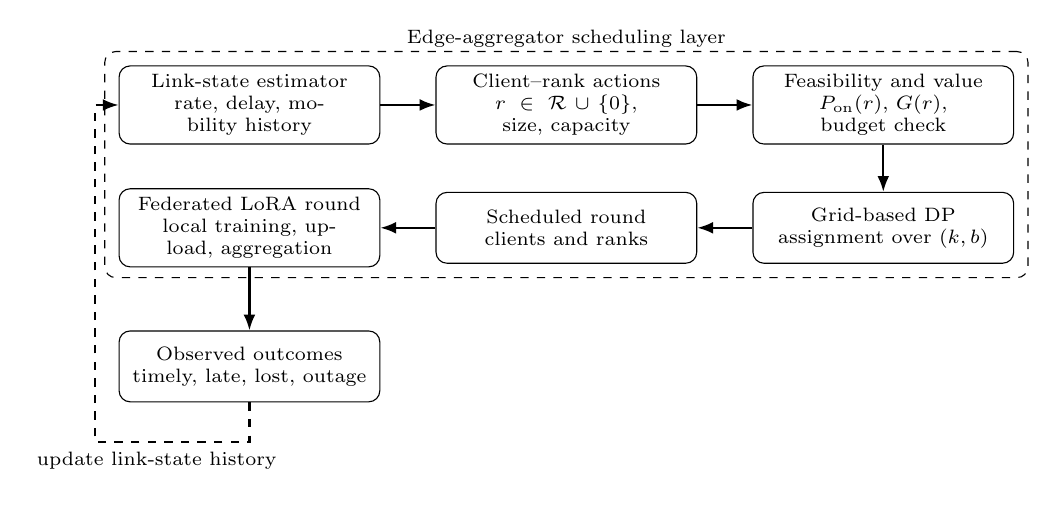
\begin{tikzpicture}[
  node distance=6mm and 7mm, >=Latex,
  box/.style={draw, rounded corners, align=center, minimum height=9mm, text width=31mm, font=\scriptsize, inner sep=3pt},
  flow/.style={-{Latex[length=2mm]}, thick},
  feedback/.style={-{Latex[length=2mm]}, dashed, thick}
]
\node[box] (estimate) {Link-state estimator\\rate, delay, mobility history};
\node[box, right=of estimate] (actions) {Client--rank actions\\$r\in\mathcal R\cup\{0\}$, size, capacity};
\node[box, right=of actions] (filter) {Feasibility and value\\$P_{\rm on}(r)$, $G(r)$, budget check};
\node[box, below=of filter] (dp) {Grid-based DP\\assignment over $(k,b)$};
\node[box, left=of dp] (assign) {Scheduled round\\clients and ranks};
\node[box, left=of assign] (fl) {Federated LoRA round\\local training, upload, aggregation};
\node[box, below=8mm of fl] (observe) {Observed outcomes\\timely, late, lost, outage};
\draw[flow] (estimate) -- (actions);
\draw[flow] (actions) -- (filter);
\draw[flow] (filter) -- (dp);
\draw[flow] (dp) -- (assign);
\draw[flow] (assign) -- (fl);
\draw[flow] (fl) -- (observe);
\coordinate (fb) at ($(fl.south)+(0,-4mm)$);
\draw[feedback] (observe.south) -- ++(0,-5mm) -| node[below, font=\scriptsize, pos=.3] {update link-state history} ($(estimate.west)+(-3mm,0)$) -- (estimate.west);
\node[draw, dashed, rounded corners, fit=(estimate)(actions)(filter)(dp)(assign), inner sep=5pt,
      label={[fill=white, inner sep=1pt, font=\scriptsize]above:Edge-aggregator scheduling layer}] {};
\end{tikzpicture}%
}
\caption{Round pipeline of FedRAS. The edge aggregator jointly selects clients and LoRA ranks with the grid-based dynamic program; only observed transmission outcomes update the link-state history.}
\label{fig:architecture}
\end{figure}

\subsection{Mobile edge FL architecture}
We consider a mobile edge network in which an edge aggregator serves a client set
$\mathcal{D}=\mathcal{D}_g\cup\mathcal{D}_a\cup\mathcal{D}_s$ of ground clients $\mathcal{D}_g$, aerial and UAV clients $\mathcal{D}_a$, and satellite-connected clients $\mathcal{D}_s$. Ground links are comparatively stable, aerial links face frequent handover, and satellite links suffer long propagation delay, intermittent visibility, and outages \cite{mahboob2024ntn,razmi2022ground}. The aggregator holds the global model, schedules every round, and aggregates the timely updates. Fig.~\ref{fig:architecture} shows the resulting round pipeline. In every round the aggregator estimates the link states, constructs and filters the client--rank actions, and solves the assignment with the grid-based dynamic program of Section~\ref{sec:solver}. It then executes the federated round and feeds the observed delivery outcomes back into the link-state history.

\subsection{Federated LoRA rounds}
Let $w^t$ denote the frozen backbone broadcast at round $t$. Client $i$ trains LoRA factors $A_{i,\ell}$ and $B_{i,\ell}$ for the adapted layers $\ell\in\mathcal L$ with layer dimensions $d_\ell\times k_\ell$. The effective weight change is $\Delta W_{i,\ell}=B_{i,\ell}A_{i,\ell}$. A rank $r$ update uses the first $r$ columns of $B_{i,\ell}$ and the first $r$ rows of $A_{i,\ell}$. A round then proceeds as follows. The aggregator broadcasts the backbone and the current adapter state. It observes the client link states and solves the client--rank assignment under the deadline, budget, and participation constraints. The admitted clients train locally and upload their rank-$r$ adapters before the deadline $\tau$. The aggregator aggregates the timely updates with data-size weights and updates its link-state history from the observed outcomes. Late or lost updates are discarded, because stale updates harm convergence stability in deadline-critical federated learning.

\subsection{Link, mobility, and delivery model}
At decision time the scheduler receives an estimated uplink rate $\bar R_i^t$ in Mbps and a mobility state. The realized rate $R_i^t$, handover event $H_i^t\in\{0,1\}$, and packet loss indicator $J_i^t$ are not observed before transmission. For an update of $B_i^t(r)$ normalized megabytes, the modeled delivery time is
\begin{equation}
T_i^t(r)=T_{\rm train,i}(r)+T_{\rm proc,i}(r)+\frac{8B_i^t(r)}{R_i^t}+d_i^t+H_i^t\Delta d_h.
\label{eq:delivery}
\end{equation}
Here the factor 8 converts megabytes to Mbit. Timely delivery is the event
\begin{equation}
P_{\rm on,i}^t(r)=\Pr\!\left(T_i^t(r)\le\tau,\;J_i^t=0\mid x_i^t\right).
\label{eq:pon}
\end{equation}

The implementation uses the following hazard surrogate rather than a derived distribution for all terms in \eqref{eq:delivery}.
\begin{equation}
\hat P_{\rm on,i}^t(r)=\exp\!\big(-\mu_i^t\big)\exp\!\Big(-\frac{8B_i^t(r)}{\bar R_i^t\tau}\Big).
\label{eq:hazard}
\end{equation}
The dimensionless intensity $\mu_i^t$ summarizes mobility related failure risk, packet loss, handover effects, and unmodeled processing time. It is not estimated by an EWMA in the present implementation. The experiments generate mobility state from the stated Beta model and provide that state and the generated rate as oracle estimates. Thus, \eqref{eq:hazard} is an idealized plug in predictor used to isolate scheduling behavior. The calibration and noise studies assess sensitivity to this predictor, but they do not constitute calibration on measured wireless traces. Training and processing times are included in the conceptual delivery model but are not separately measured in the current experiments.

\subsection{Rank-dependent update size and capacity}
With $b$ bits per parameter, the payload of a rank-$r$ LoRA update is
\begin{equation}
B_i^t(r)=\frac{b}{8}\;r\!\!\sum_{\ell\in\mathcal L}\big(d_\ell+k_\ell\big)+B_{\rm meta},
\label{eq:size}
\end{equation}
in MB, where $B_{\rm meta}$ covers headers and metadata. Rank is therefore a network-visible resource. It scales both the adaptation capacity and the transmission time. We model the useful contribution of a delivered rank-$r$ update with the saturating capacity gain
\begin{equation}
G_i^t(r)=\pi_i^t\,\sqrt{\min(r,r_{\max})/r_{\max}},
\label{eq:cap}
\end{equation}
where $\pi_i^t$ is a per-client contribution prior in the spirit of Oort-style utility \cite{oort2021oort}. In the simulator, this prior is sampled from a stated uniform range; in the real trainer, data size and update norms are used for aggregation and the Oort-style baseline, while the FedRAS rank rule uses the capacity--delivery score. The width $r_{\max}$ is the factor width provisioned at all clients. The square root encodes diminishing returns of rank. The saturation at $r_{\max}$ reflects that wider factors add payload but no expressible capacity once the provisioned width is reached. The full-parameter FedAvg updates of our experiments are represented by a rank-64 payload in the simulator.

\section{Deadline-aware client--rank scheduling}
\label{sec:problem}

Each round, the aggregator decides $a_i^t\in\{0\}\cup\mathcal R$, where $a_i^t=0$ means client $i$ does not participate and $a_i^t=r$ schedules it at rank $r$. The per-round problem is
\begin{equation}
\max_{\{a_i^t\}}\;\sum_{i\in\mathcal D}\mathbf 1\{a_i^t>0\}\,G_i^t(a_i^t)\,P_{\rm on,i}^t(a_i^t)
\label{eq:objective}
\end{equation}
\begin{equation}
\text{s.t.}\quad \sum_i B_i^t(a_i^t)\le B_{\max},\qquad \sum_i\mathbf 1\{a_i^t>0\}\le K .
\label{eq:constraints}
\end{equation}
The objective is a scheduling utility. It counts expected useful delivered updates under the byte budget $B_{\max}$ and participation cap $K$. It is not a direct surrogate for final test accuracy. Increasing $r$ raises $G$ sublinearly, increases payload, and lowers the delivery surrogate. The experiments therefore report test accuracy, timely delivery ratio, bytes per round, and mean delivered rank as separate outcomes.

Two deployment variants are evaluated. In full grid scheduling, the aggregator solves \eqref{eq:objective} and \eqref{eq:constraints} over all clients. The solver study evaluates this variant at 500-client scale. In the real trainer, fair-cohort scheduling samples the fixed cohort of ten clients and applies the per-client rank rule $r_i^\star=\arg\max_r G_i^t(r)P_{\rm on,i}^t(r)$. The byte budget is enforced only by the full grid-scheduling arm, while bytes are reported for all methods. Section~\ref{sec:dpvfair} compares the variants in the trainer.

\section{Grid-based solver and heterogeneous-rank aggregation}
\label{sec:solver}

\subsection{Dynamic program}
Problem \eqref{eq:objective}--\eqref{eq:constraints} is a multiple-choice knapsack with an admission constraint. Let $q=0.05$ MB be the budget grid and define the integer cost $\widetilde B_i(r)=\operatorname{round}(B_i^t(r)/q)$. Let $V_i(k,b)$ be the maximum estimated utility from the first $i$ clients with $k$ admissions and integer budget $b$. Initialize $V_0(0,0)=0$ and all other states to $-\infty$. The recurrence is
\begin{equation}
V_i(k,b)=\max\Big\{V_{i-1}(k,b),\;\max_{r\in\mathcal R}\big[V_{i-1}(k-1,b-\widetilde B_i(r))+u_i(r)\big]\Big\},
\label{eq:dp}
\end{equation}
where $u_i(r)=G_i^t(r)\hat P_{\rm on,i}^t(r)$. Backpointers recover the assignment.

\begin{proposition}[Per-round optimality]
For every reachable state $(k,b)$, recurrence \eqref{eq:dp} considers the skip action and every feasible rank for client $i$. Induction on $i$ therefore proves exactness for the discretized single round estimated assignment problem. The result is not a claim of optimality for the continuous budget problem, the multi-round stochastic control problem, or final model accuracy.
\end{proposition}
\begin{proof}
The admission indicator and the rank of each client are exclusive actions that affect the two resources additively. Admitting client $i$ at rank $r$ consumes one admission slot and $B(r)$ budget units and adds $u_i(r)$ value, independent of the other clients. The state $(k,b)$ therefore summarizes all interaction, and the standard interchange argument for the multiple-choice knapsack applies. Any optimal solution restricted to the first $i-1$ clients must itself be optimal for its state, which the recurrence maximizes.
\end{proof}

The complexity is $O(|\mathcal D|K\widetilde B_{\max}|\mathcal R|)$ time and $O(K\widetilde B_{\max})$ memory with rolling arrays, where $\widetilde B_{\max}=B_{\max}/q$. The implementation uses $q=0.05$ MB. Section~\ref{sec:dp_study} reports the resulting runtimes for 500 and 1000 clients.

\begin{algorithm}[t]
\caption{FedRAS scheduling round}
\label{alg:scheduler}
\begin{algorithmic}[1]
\REQUIRE clients $\mathcal D$, ranks $\mathcal R$, cap $K$, budget $B_{\max}$, deadline $\tau$, states $\{x_i^t\}$
\ENSURE admitted set and assigned ranks
\STATE Estimate $\hat P_{\rm on,i}^t(r)$ by \eqref{eq:hazard} and $G_i^t(r)$ by \eqref{eq:cap} for all $i,r$
\STATE Initialize $V_0(0,0)=0$; other DP states to $-\infty$
\FOR{each client $i\in\mathcal D$}
  \FOR{$k=0,\dots,K$ and each budget state $b$}
    \STATE Apply skip and every feasible rank transition of \eqref{eq:dp}
    \STATE Store the maximizing action as a backpointer
  \ENDFOR
\ENDFOR
\STATE Backtrack from $\max_{k,b} V_{|\mathcal D|}(k,b)$; return the client--rank assignment
\STATE Execute the round; aggregate timely rank-masked updates (Section~\ref{sec:aggregation}); update link-state history
\end{algorithmic}
\end{algorithm}

\subsection{Rank-masked aggregation with frozen factors}
\label{sec:aggregation}
Clients scheduled at different ranks share an $r_{\max}$ coordinate system. For one adapted layer, client $i$ has sample weight $n_i$ and delivered rank $r_i$. The factor $A\in\mathbb R^{r_{\max}\times k}$ is frozen and shared, while $B_i\in\mathbb R^{d\times r_{\max}}$ is trainable. A rank $r_i$ update activates columns $1$ through $r_i$ of $B_i$ and the matching rows of $A$, giving $\Delta W_i=\sum_{j\le r_i}[B_i]_{:,j}[A]_{j,:}$.

Jointly trained factor pairs $(A_i,B_i)$ are identifiable only up to invertible transforms, so separately averaged factors need not average the updates at all. Section~\ref{sec:eval} quantifies this failure mode in an ablation.

\textbf{Rank-masked averaging.} The server zero-pads inactive columns of each delivered $B_i$ and averages each active coordinate over the clients that activate it,
\begin{equation}
\bar B_{:,j}=\frac{1}{W_j}\sum_{i:\,r_i\ge j} n_i\,\big[B_i\big]_{:,j},
\qquad
W_j=\sum_{i:\,r_i\ge j} n_i ,
\label{eq:maskavg}
\end{equation}
while the frozen factor aggregates to itself, $\bar A=A$. The server then applies momentum per factor tensor. With $\Delta^t=\bar B-S^{t-1}$, the velocity and state update as $v^t=\beta\,v^{t-1}+(1-\beta)\,\Delta^t$ and $S^t=S^{t-1}+v^t$, with $\beta=0.3$ damping client-sampling and link noise.

\begin{proposition}[Exactness of frozen-factor aggregation]
\label{prop:agg}
Under \eqref{eq:maskavg}, the $j$-th active rank slice of $\bar BA$ is the data-weighted average over clients with $r_i\ge j$. This is exact coordinate-wise averaging of active induced-update slices. It is not, in general, the unified data-weighted average of complete client updates. If a common denominator $W=\sum_i n_i$ is used instead of $W_j$, the unified average is recovered, but active high-rank slices are diluted by $W_j/W$. The two rules coincide for all possible updates when all delivered ranks are equal.
\end{proposition}
\begin{proof}
The first two parts follow from linearity. For frozen shared $A$, multiplying a weighted sum of $B$-coordinates by $\big[A\big]_{j,:}$ converts it into the same weighted sum of the matching update slices, and the two normalizers differ only in $W_j$ versus $W$. The product $\bar BA=\sum_j\bar B_{:,j}\big[A\big]_{j,:}$ collects the slices. The third part holds because $W_j=W$ for every active $j$ if and only if $r_i=\max_k r_k$ for all admitted $i$ with $n_i>0$.
\end{proof}

The proposition concerns active rank slices rather than whole-update equivalence. With shared frozen $A$, it gives coordinate-wise data-weighted averaging and avoids dilution caused by a common denominator. The elevated-learning-rate ablation tests the associated stability claim. It does not establish a general convergence guarantee.

\section{Performance evaluation}
\label{sec:eval}

The evaluation tests accuracy and network behavior in a real trainer, scheduling quality at 500 clients, solver cost, and sensitivity to payload, predictor, capacity, and budget-grid assumptions.

\subsection{Experimental setup}
\textbf{Real trainer.} The trainer is implemented in PyTorch and runs on one A800 GPU. The backbone is a six-convolution BatchNorm CNN with channel progression 64/128/256, followed by two 256-wide linear layers. It is centrally pretrained with crop, flip, and erase augmentation, Nesterov momentum, weight decay, and cosine learning-rate decay, for 30 epochs on CIFAR-10, 45 on CIFAR-100, and 3 on MNIST, and then frozen. LoRA adapters with candidate rank set $\mathcal R=\{2,4,8,16\}$ and provisioned width $r_{\max}=16$ are placed on all six convolutions through 1$\times$1 factors and on both head layers, so the rank genuinely bounds the capacity of every adapted weight. The pretrained backbone reaches a test accuracy of 0.914 on CIFAR-10, 0.692 on CIFAR-100, and 0.995 on MNIST.

\textbf{Federated protocol and links.} The real trainer uses 20 clients partitioned with Dirichlet $\alpha=0.5$, 10 sampled participants per round, one local epoch, batch size 128, and 40 rounds. The candidate ranks are $\{2,4,8,16\}$ with $r_{\max}=16$. Local SGD uses learning rate 0.005, weight decay $10^{-4}$, gradient clipping at 1, and cosine decay. The server uses rank-masked weighted averaging with momentum 0.3. Results use five seeds, 0 through 4, unless a caption states ten seeds. The rate is LogNormal$(2.5,0.7)$ clipped to $[1,40]$ Mbps, and mobility is Beta$(2,5)$ redrawn each round. These generated states are supplied as oracle estimates to the scheduler. Predictor noise and calibration variants are evaluated separately.

\begin{table}[H]
\centering
\caption{Payload audit of the actual serialized adapter-update size against the stylized payload model $s(r)$. The frozen backbone (1.28\,M parameters) is 5.13\,MB in FP32; factor shapes are listed in the reproducibility package.}
\label{tab:audit}
\resizebox{\columnwidth}{!}{%
\begin{tabular}{lccc}
\toprule
Rank $r$ & Actual FP32 (MB) & Actual FP16 (MB) & Stylized $s(r)$ (MB)\\
\midrule
2  & 0.010 & 0.005 & 0.54\\
4  & 0.021 & 0.010 & 0.58\\
8  & 0.041 & 0.021 & 0.66\\
16 & 0.082 & 0.041 & 0.82\\
64 (full-update representation) & 0.328 & 0.164 & 1.78\\
\bottomrule
\end{tabular}%
}
\end{table}

\textbf{Model and payload audit.} The simulator uses $s(r)=0.02r+0.5$ normalized MB per client and represents full updates by rank 64. The eight adapter layers contain 1{,}283 factor parameters per rank column, or 10.25\,KB in FP32. A rank-16 update is 0.082\,MB when serialized, while the stylized model adds a common 0.5\,MB allowance and a larger rank-dependent slope. This common convention preserves cross-method byte comparisons.

Full-parameter updates train the entire backbone plus the head adapters, 5.21\,MB per client in FP32, so the rank-64 representation understates their byte bill by $2.9\times$. This bias favors FedAvg, and at the true FP32 size its timely delivery ratio would decrease further than reported.

\textbf{Simulator.} The 500-client, 150-round simulation uses the same delivery and capacity models with uniform cohort sampling, per-client rank selection, and budget admission. It covers nominal, deadline, budget, mobility, and 1000-client scalability regimes, with five seeds and common traces.

\textbf{Scoring proxy.} The simulator samples $\pi_i$ uniformly from $[0.15,0.45]$ and uses a bounded scheduling proxy rather than dataset accuracy. Starting at 0.1, it updates as $a^{t+1}=a^t+\eta\hat g^t(1-a^t)-\varepsilon a^t$, where $\hat g^t$ is useful delivered value normalized by $K$, $\eta=0.08$, and $\varepsilon=0.0005$.
\textbf{Solver study.} The solver study runs 30 instances per deadline and budget cell at 500 clients. It compares the grid-based DP with value-per-byte greedy, value greedy, and fixed rank 16, and adds a client-count sweep that extends to 1000 clients in size.
All trainer methods use the same client partitions, local optimizer, rank set where applicable, generated rate and mobility states, deadline, and seed protocol. The full-parameter baseline uses the same local training schedule and differs in the transmitted parameter set. Communication metrics count attempted uplink bytes, including late and failed uploads. No quantization, sparsification, energy, or fairness metric is claimed in this study.

\begin{figure}[H]
\centering
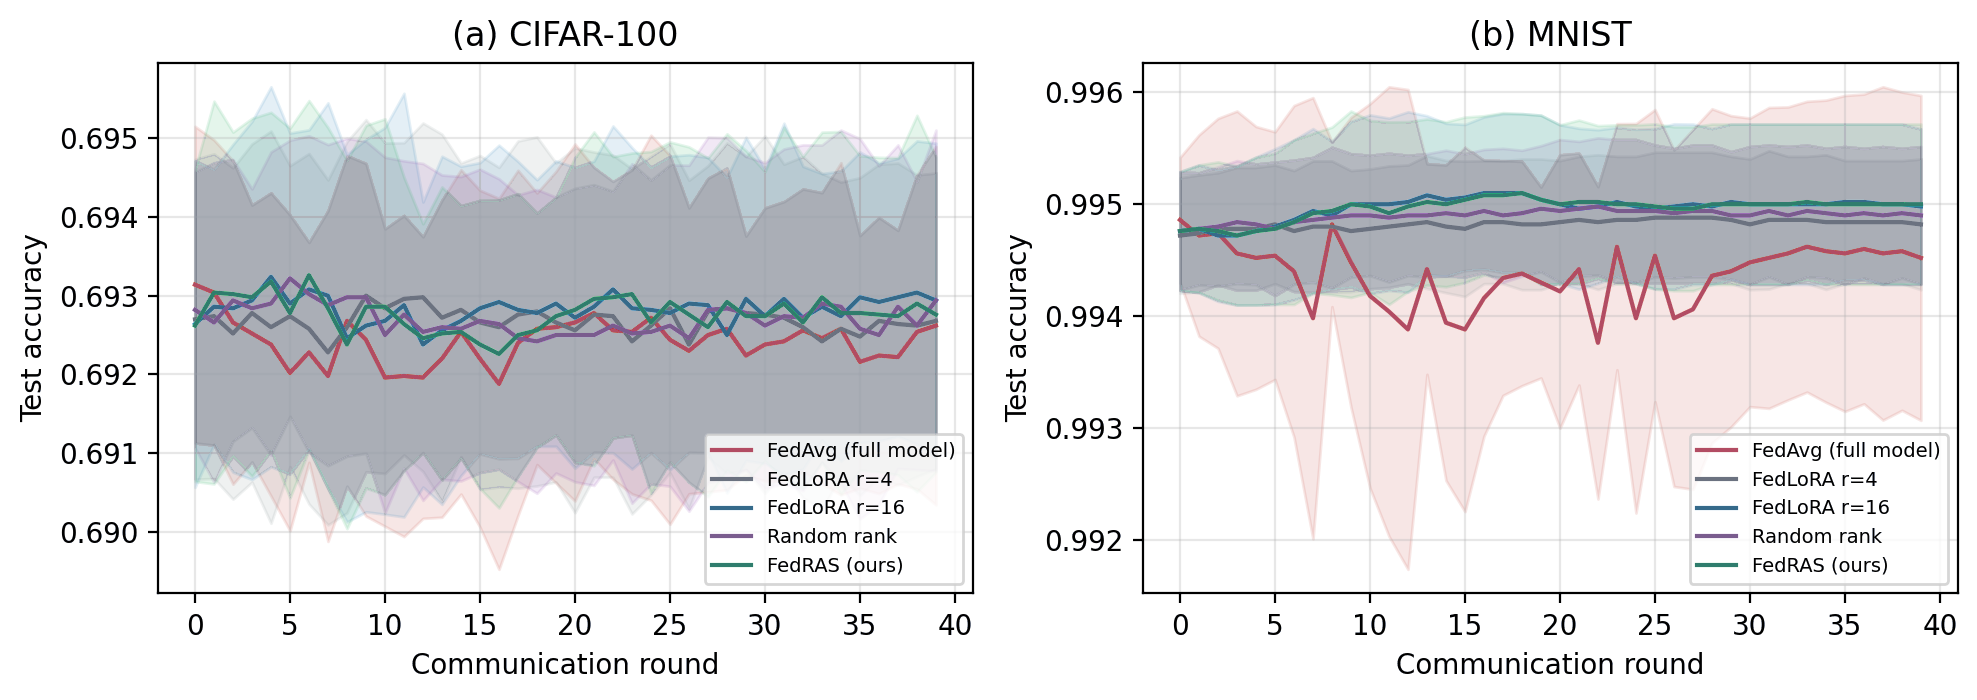
\includegraphics[width=0.8\columnwidth]{recolored_figures/cross_dataset.png}
\caption{Cross-dataset test accuracy on CIFAR-100 and MNIST. Values are mean$\pm$std over five seeds. The parity and stability findings of Table~\ref{tab:trainer} are not CIFAR-10-specific.}
\label{fig:crossds}
\end{figure}

\begin{table}[H]
\centering
\caption{Real trainer on non-IID CIFAR-10 with five seeds. Accuracy is measured at round 40. Timely delivery ratio is timely deliveries divided by selected clients. Bytes per round is the sum of attempted uplink payloads for selected clients over rounds 30 to 39. Failed or late uploads remain included. Mean rank is computed over delivered updates. Acc/MB is round-40 accuracy divided by bytes per round.}
\label{tab:trainer}
\resizebox{0.92\columnwidth}{!}{%
\begin{tabular}{lccccc}
\toprule
Method & Accuracy & Timely delivery ratio & Bytes/round & Mean rank & Acc/MB ($\times10^{-2}$)\\
\midrule
FedAvg (full model) & $0.9138\pm0.0019$ & 0.28 & 17.80 & 64 & 5.1\\
FedLoRA $r{=}4$ & $0.9145\pm0.0012$ & 0.50 & 5.80 & 4 & 15.8\\
FedLoRA $r{=}16$ & $0.9142\pm0.0016$ & 0.44 & 8.20 & 16 & 11.1\\
Random rank & $0.9144\pm0.0016$ & 0.49 & 6.51 & 7.4 & 14.1\\
FedRAS (ours) & $0.9143\pm0.0015$ & 0.44 & 8.14 & 16.0 & 11.2\\
\bottomrule
\end{tabular}%
}
\end{table}

\subsection{Accuracy parity and rank invariance in the trainer}
Table~\ref{tab:trainer} reports five-seed means and standard deviations after 40 federated rounds on CIFAR-10. All LoRA methods hold the backbone accuracy within one standard deviation of 0.914, whether the rank is fixed at 4, fixed at 16, drawn at random, or selected by the rank rule. Full-parameter updates also match this accuracy, but they spend 17.8 normalized MB per round against 5.8 to 8.2 for the LoRA ranks, a factor of 2.2 to 3.1. They also lose roughly half of the timely deliveries, 0.28 against 0.44 to 0.50, because their large payloads are dropped more often. The trainer shows no measurable accuracy difference in this setting. With a frozen pretrained backbone, the observed differences are on the network side. The cross-dataset results agree at 0.693 on CIFAR-100 and 0.995 on MNIST. Figs.~\ref{fig:crossds} and \ref{fig:trainer_acc} show the corresponding trajectories, all stable over the 40 rounds for every rank policy.

\begin{figure}[H]
\centering
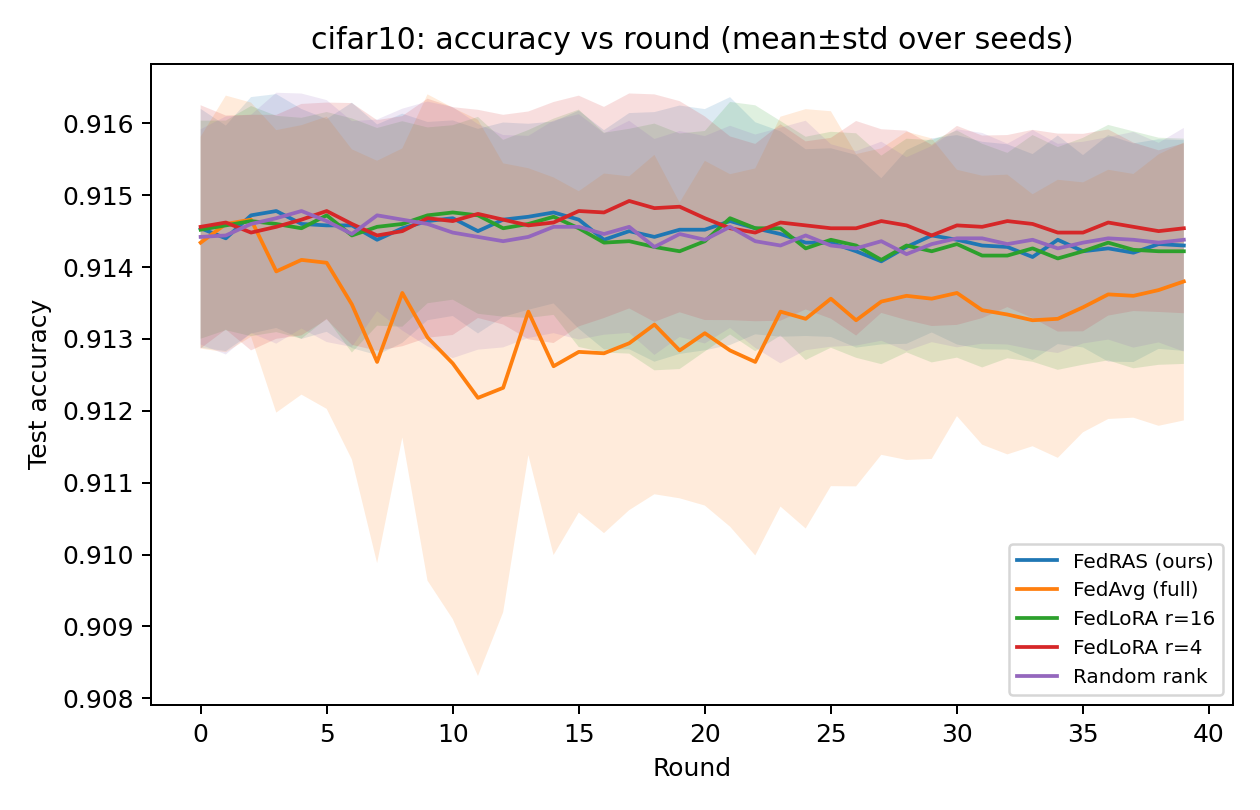
\includegraphics[width=0.8\columnwidth]{trainer_accuracy.png}
\caption{Real-trainer CIFAR-10 test accuracy over 40 federated rounds (mean$\pm$std over five seeds). All rank policies hold the pretrained-backbone accuracy; differences appear in bytes and timeliness, not accuracy.}
\label{fig:trainer_acc}
\end{figure}

\subsection{Deadline stress in the trainer}
Table~\ref{tab:stress} tightens the deadline to 0.5\,s and 0.25\,s with five seeds. It reports accuracy at round 40 and network metrics averaged over rounds 30 to 39. Three effects emerge. First, FedRAS downshifts under pressure. Its delivered mean rank falls from 16.0 at the nominal deadline to 15.5 at 0.5\,s and 13.5 at 0.25\,s, where the delivery hazard \eqref{eq:hazard} makes rank-16 payloads marginal. The loose-deadline control at 2\,s in Table~\ref{tab:extended} restores rank 16.0, so FedRAS upshifts again when pressure is absent. Second, downshifting pays. FedRAS matches the accuracy of fixed $r{=}16$, 0.9145 versus 0.9142, while transmitting 14\% fewer bytes, 7.07 against 8.20\,MB, and achieving a similar timely delivery ratio. Third, full-parameter updates collapse. Their timely delivery ratio falls from 0.28 at the nominal deadline in Table~\ref{tab:trainer} to 0.13 at 0.5\,s and 0.04 at 0.25\,s, so only 0.4 of the 10 updates arrive per round at an unchanged $2.2\times$ byte cost.

\begin{table}[H]
\centering
\caption{Extended stress matrix. Results use five seeds and report round-40 accuracy as mean$\pm$std. The loose-deadline and mobility-only scenarios confirm that FedRAS upshifts when pressure is absent; $\alpha{=}0.1$ probes extreme non-IID heterogeneity; the last two columns repeat the 0.25\,s deadline on CIFAR-100 and MNIST. Bold marks the best value at displayed precision, ties included.}
\label{tab:extended}
\resizebox{0.92\columnwidth}{!}{%
\begin{tabular}{l ccccc}
\toprule
Method & dl 2\,s & Mob.\ 0.7 & $\alpha{=}0.1$ & CIFAR-100 dl 0.25\,s & MNIST dl 0.25\,s\\
\midrule
FedAvg (full model) & $0.9128\pm.0026$ & $0.9125\pm.0016$ & $0.9059\pm.0047$ & $0.6924\pm.0021$ & $0.9946\pm.0009$\\
FedLoRA $r{=}4$ & $\mathbf{0.9144\pm.0013}$ & $0.9143\pm.0015$ & $\mathbf{0.9138\pm.0014}$ & $\mathbf{0.6928\pm.0022}$ & $0.9948\pm.0006$\\
FedLoRA $r{=}16$ & $\mathbf{0.9144\pm.0015}$ & $0.9142\pm.0014$ & $0.9109\pm.0026$ & $0.6927\pm.0017$ & $\mathbf{0.9949\pm.0006}$\\
Random rank & $\mathbf{0.9144\pm.0016}$ & $0.9142\pm.0019$ & $\mathbf{0.9140\pm.0018}$ & $\mathbf{0.6928\pm.0020}$ & $\mathbf{0.9949\pm.0007}$\\
FedRAS (ours) & $0.9142\pm.0014$ & $\mathbf{0.9143\pm.0015}$ & $0.9111\pm.0028$ & $0.6925\pm.0020$ & $\mathbf{0.9949\pm.0006}$\\
\bottomrule
\end{tabular}%
}
\end{table}

\begin{table}[H]
\centering
\caption{Real trainer under deadline stress with five seeds. Accuracy is the round-40 mean and standard deviation. Timely delivery ratio, bytes per round, and mean delivered rank are averaged over rounds 30 to 39. Bytes count attempted uplink payloads for selected clients.}
\label{tab:stress}
\resizebox{0.92\columnwidth}{!}{%
\begin{tabular}{l cccc cccc}
\toprule
& \multicolumn{4}{c}{deadline 0.5\,s} & \multicolumn{4}{c}{deadline 0.25\,s}\\
\cmidrule(lr){2-5}\cmidrule(lr){6-9}
Method & Acc. & Timely delivery ratio & Bytes & Rank & Acc. & Timely delivery ratio & Bytes & Rank\\
\midrule
FedAvg (full model) & $0.9132\pm.0021$ & 0.13 & 17.80 & 64 & $0.9137\pm.0026$ & 0.04 & 17.80 & 64\\
FedLoRA $r{=}4$ & $0.9142\pm.0013$ & 0.37 & 5.80 & 4 & $0.9147\pm.0019$ & 0.21 & 5.80 & 4\\
FedLoRA $r{=}16$ & $0.9141\pm.0015$ & 0.30 & 8.20 & 16 & $0.9142\pm.0019$ & 0.15 & 8.20 & 16\\
Random rank & $0.9143\pm.0014$ & 0.32 & 6.51 & 6.5 & $0.9148\pm.0017$ & 0.17 & 6.51 & 6.5\\
FedRAS (ours) & $0.9141\pm.0018$ & 0.31 & 7.80 & 15.5 & $0.9145\pm.0020$ & 0.16 & 7.07 & 13.5\\
\bottomrule
\end{tabular}%
}
\end{table}

Accuracy spreads remain within about two standard deviations, which is consistent with the parity claim. The scheduling metrics are where the methods separate. Fig.~\ref{fig:trainer_dl} shows the five-seed stress trajectories. Fig.~\ref{fig:rankdyn} visualizes the mechanism directly. The delivered rank of FedRAS sits at 16 under the nominal deadline, dips under the 0.5\,s deadline, and tracks 10 to 14 under the 0.25\,s deadline, whereas the annealed baseline follows its fixed heat--cool path regardless of link state. A ten-seed replication confirms these differences at conventional significance levels, with full statistics in Section~\ref{sec:summary}. Under the 0.25\,s deadline, FedRAS transmits 14.5\% fewer bytes than fixed $r{=}16$, with a seed-mean bootstrap 95\% confidence interval from 12.4\% to 18.6\% and a two-sided Wilcoxon $p$ of 0.002. It delivers a higher timely delivery ratio in ten of ten seed pairs at $p=0.016$, and it remains statistically indistinguishable in accuracy at $p=0.40$.

\begin{figure}[H]
\centering
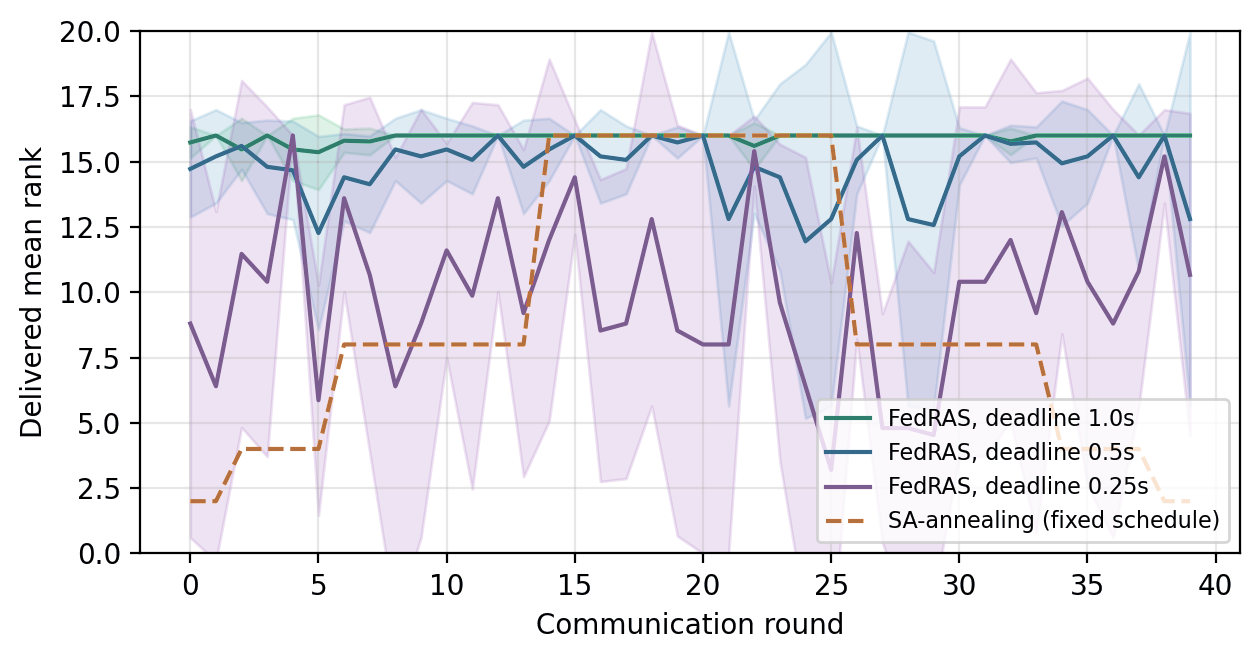
\includegraphics[width=0.8\columnwidth]{recolored_figures/rank_dynamics.png}
\caption{Delivered mean rank per round for FedRAS under three deadlines (mean$\pm$std, five seeds), against the fixed annealing schedule of the SA-FedLoRA-style baseline. FedRAS is link-aware, holding high rank when possible and downshifting under pressure.}
\label{fig:rankdyn}
\end{figure}

\begin{figure}[H]
\centering
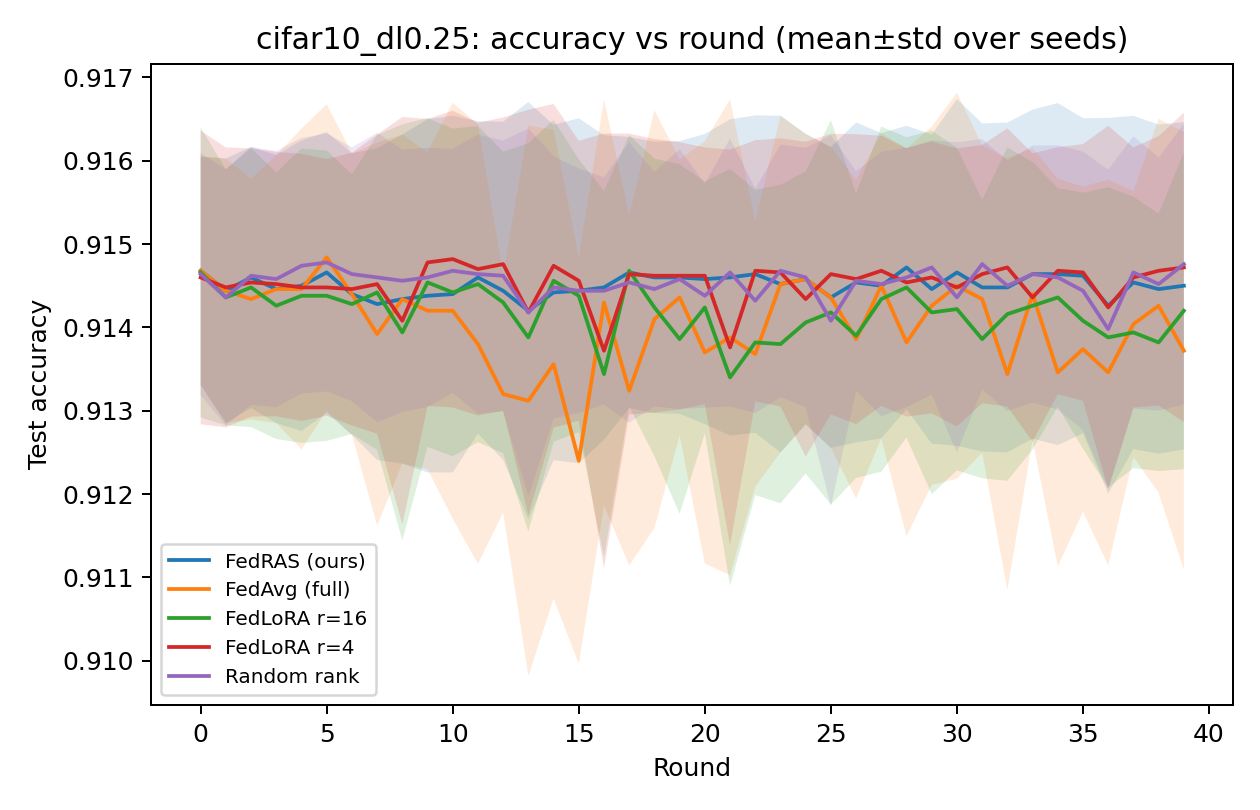
\includegraphics[width=0.8\columnwidth]{trainer_dl025.png}
\caption{Real-trainer accuracy trajectories under the 0.25\,s deadline (mean$\pm$std, five seeds). All methods remain stable. FedRAS selects lower ranks on slow links and matches rank-16 delivery at 14\% fewer bytes.}
\label{fig:trainer_dl}
\end{figure}

\subsection{Broader stress matrix with mobility, heterogeneity, and cross-dataset checks}
Table~\ref{tab:extended} extends the stress study along three further axes. A mobility-only scenario with Beta$(0.7,\,5)$ mobility and the nominal deadline leaves FedRAS at the top rank and at parity, so mobility alone does not force downshifting at this deadline, consistent with the mobility-stress regime of the simulator. Extreme label heterogeneity with $\alpha{=}0.1$ reveals a second-order effect. Rank-16 updates lose about 0.3 points relative to rank 4, 0.9109 versus 0.9138, which is consistent with capacity-amplified client drift, and full-parameter updates lose the most at 0.9059. FedRAS follows the rank-16 trajectory here, so a heterogeneity-aware downshift is a natural extension. Repeating the 0.25\,s deadline on CIFAR-100 and MNIST reproduces the CIFAR-10 stress picture, with parity across LoRA ranks and a timely delivery ratio of 0.04 for full-parameter updates, meaning 0.4 of 10 updates per round. The scheduling conclusions are therefore not dataset-specific.

\subsection{External baselines and component ablations}
Table~\ref{tab:ext} adds three external baselines to the trainer. The first is an SA-FedLoRA-style schedule that heats the rank from 2 to 16 and cools it down over the 40 rounds, oblivious to link state \cite{yang2024safedlora}. The second is an Oort-style selector that samples $2K$ candidates and admits the top-$K$ by a data-size-and-recency utility at fixed rank \cite{oort2021oort}. The third is joint A/B training with plain averaging, the aggregation-level competitor of Section~\ref{sec:aggregation} \cite{guo2025fedsalora}.

\begin{table}[H]
\centering
\caption{External baselines in the real trainer on non-IID CIFAR-10 with five seeds. Accuracy is measured at round 40. Timely delivery ratio, bytes, and delivered mean rank are averaged over rounds 30--39.}
\label{tab:ext}
\resizebox{\columnwidth}{!}{%
\begin{tabular}{l cccc cccc}
\toprule
& \multicolumn{4}{c}{nominal deadline} & \multicolumn{4}{c}{deadline 0.25\,s}\\
\cmidrule(lr){2-5}\cmidrule(lr){6-9}
Method & Acc. & Timely delivery ratio & Bytes & Rank & Acc. & Timely delivery ratio & Bytes & Rank\\
\midrule
SA-FedLoRA-style annealing & $0.9145\pm.0016$ & 0.49 & 6.04 & 5.2 & $0.9146\pm.0016$ & \textbf{0.20} & \textbf{6.04} & 4.8\\
Oort-style utility, fixed rank & $0.9141\pm.0017$ & 0.49 & 6.60 & 8.0 & $0.9142\pm.0013$ & 0.18 & 6.60 & 6.4\\
Joint A/B, plain averaging & $0.9143\pm.0015$ & 0.44 & 8.20 & 16 & $0.9140\pm.0017$ & 0.15 & 8.20 & 12.5\\
\midrule
FedLoRA $r{=}16$ & $0.9142\pm.0016$ & 0.44 & 8.20 & 16 & $0.9142\pm.0019$ & 0.15 & 8.20 & 12.5\\
FedRAS (ours) & $0.9143\pm.0015$ & 0.44 & 8.14 & 16.0 & $0.9145\pm.0020$ & 0.16 & 7.07 & 13.5\\
\bottomrule
\end{tabular}%
}
\end{table}

\begin{table}[H]
\centering
\caption{Scheduler simulation with 500 clients, 150 rounds, and five seeds. The accuracy column is a bounded scheduling proxy, not dataset accuracy. Timely delivery ratio is the mean delivery probability for admitted clients, and bytes are the attempted uplink payload total for admitted clients in the final round.}
\label{tab:sim}
\resizebox{0.92\columnwidth}{!}{%
\begin{tabular}{lccc ccc ccc ccc}
\toprule
& \multicolumn{3}{c}{Nominal} & \multicolumn{3}{c}{Deadline 0.25\,s} & \multicolumn{3}{c}{Budget 12 MB} & \multicolumn{3}{c}{1000 clients}\\
\cmidrule(lr){2-4}\cmidrule(lr){5-7}\cmidrule(lr){8-10}\cmidrule(lr){11-13}
Method & Acc. & Timely delivery ratio & Bytes & Acc. & Timely delivery ratio & Bytes & Acc. & Timely delivery ratio & Bytes & Acc. & Timely delivery ratio & Bytes\\
\midrule
FedAvg & .607 & .26 & 44.5 & .187 & .04 & 44.5 & .397 & .43 & 10.7 & .577 & .35 & 58.7\\
$r{=}4$ & .606 & .51 & 14.5 & .343 & .20 & 14.5 & .576 & .54 & 11.6 & .610 & .51 & 29.0\\
$r{=}16$ & \textbf{.778} & .44 & 20.5 & .404 & .14 & 20.5 & \textbf{.687} & .52 & 11.5 & \textbf{.781} & .44 & 41.0\\
Random & .666 & .48 & 16.5 & .359 & .18 & 16.5 & .620 & .52 & 11.9 & .668 & .48 & 32.9\\
Reliability-only & .508 & .52 & 13.5 & .292 & .22 & 13.5 & .493 & .55 & 11.9 & .511 & .52 & 27.0\\
SA-FedLoRA-style annealing & .696 & .52 & 13.5 & .374 & .22 & 13.5 & .636 & .55 & 11.9 & .699 & .52 & 27.0\\
FedRAS (ours) & \textbf{.778} & .44 & 20.3 & \textbf{.413} & .15 & 17.8 & \textbf{.687} & .52 & 11.5 & \textbf{.781} & .44 & 40.7\\
\bottomrule
\end{tabular}%
}
\end{table}

All methods remain close to the backbone accuracy in this proxy study. The differences are network-side. At 0.25\,s, the link-oblivious annealing schedule remains at low rank and delivers more updates at fewer bytes, but it cannot increase rank when links improve. Its proxy accuracy is 0.696 versus 0.778 for FedRAS in the nominal regime and 0.374 versus 0.413 under stress.

The Oort-style selector prioritizes high-utility clients at fixed rank. Joint A/B training matches frozen-factor training at the adopted learning rate, but its stability cost appears under elevated learning rate.

A ten-seed replication of the three baselines under both deadlines confirms this picture at conventional significance levels. No measurable accuracy difference was detected, with a largest mean difference of 0.03 percentage points and all $p\ge0.09$. The annealed schedule reaches higher timely delivery ratios at fewer bytes, exactly as its fixed low-rank path predicts, with $p\le0.004$. Oort-style selection saves bytes at parity with $p=0.002$. Joint A/B matches frozen-factor training in accuracy while losing timely deliveries to FedRAS under stress, by 0.019 at $p=0.016$.

\begin{table}[H]
\centering
\caption{Component ablations, real trainer (non-IID CIFAR-10, five seeds, nominal deadline). The Min. column is the minimum per-seed-mean accuracy over rounds, reported for the elevated-learning-rate stability check at lr $0.02$.}
\label{tab:ablation}
\resizebox{\columnwidth}{!}{%
\begin{tabular}{l cccc c}
\toprule
Configuration & Acc. & Timely delivery ratio & Bytes & Rank & Min.\\
\midrule
Full system (ours) & $0.9143\pm.0015$ & 0.44 & 8.14 & 16.0 & ---\\
\midrule
w/o capacity term & $0.9145\pm.0015$ & \textbf{0.52} & \textbf{5.40} & 2.0 & ---\\
w/o frozen A (joint A/B) & $0.9143\pm.0015$ & 0.44 & 8.20 & 16.0 & ---\\
w/o rank mask (mixed-rank rounds) & $0.9145\pm.0016$ & 0.49 & 6.51 & 7.4 & ---\\
w/o server momentum & $0.9144\pm.0016$ & 0.44 & 8.14 & 16.0 & ---\\
\midrule
frozen A, lr $0.02$ & $0.9128\pm.0017$ & --- & --- & --- & \textbf{0.909}\\
joint A/B, lr $0.02$ & $0.9127\pm.0017$ & --- & --- & --- & 0.901\\
\bottomrule
\end{tabular}%
}
\end{table}

Table~\ref{tab:ablation} reports component ablations. In the parity regime, no removal measurably changes final accuracy, which is consistent with the claim that accuracy is carried by the backbone and not by the scheduler. The components instead shape network behavior and stability margins. Removing the capacity term collapses FedRAS to rank 2, with 5.40 bytes and delivered rank 2.0. Delivery-only optimization is the degenerate policy that the capacity term exists to prevent. Its capacity cost is invisible at nominal deadlines but material in the simulator, where rank 2 loses 27 points of scheduling accuracy to rank 16, as Table~\ref{tab:sim} shows.

Removing the frozen-factor property does not hurt at the adopted learning rate. At an elevated rate of 0.02, joint A/B training shows a markedly deeper transient accuracy dip before recovering, with a minimum of 0.901 against 0.909 across rounds and seeds, which matches the factor-rotation analysis of Section~\ref{sec:aggregation}. The rank mask and server momentum are accuracy-neutral here, because at the adopted operating point all clients often share one rank and the momentum is small. The mask is nonetheless what keeps heterogeneous-rank aggregation per-slice exact whenever ranks mix, as Proposition~\ref{prop:agg} states.

\subsection{Full grid scheduling versus fair-cohort in the trainer}
\label{sec:dpvfair}
The trainer results so far use fair-cohort scheduling. The server samples the fixed cohort of ten clients and assigns each candidate its locally optimal rank. This arm does not apply a byte-based admission step. The full grid-based client--rank DP, by contrast, has so far been exercised only in the simulator. We therefore add a full grid-scheduling arm to the trainer. Each round, this arm solves the grid-based DP of Section~\ref{sec:solver} over the entire 20-client population, so both arms see the same candidate set. Both arms share the participation cap $K{=}10$, and the DP arm additionally enforces a byte budget of 8.2\,MB, which is $10\times$ the rank-16 payload, so the budget binds only through downshifting or skipping. The budget grid is the 0.05\,MB grid of the solver study.

\begin{table}[H]
\centering
\caption{Full grid scheduling versus fair-cohort in the real trainer on non-IID CIFAR-10 with a nominal deadline and ten seeds. Accuracy is measured at round 40 and network metrics are averaged over rounds 30--39. Both arms share all 20 clients and the participation cap $K{=}10$. The DP arm additionally enforces an 8.2\,MB byte budget.}
\label{tab:dpvfair}
\resizebox{\columnwidth}{!}{%
\begin{tabular}{lcccc}
\toprule
Method & Accuracy & Timely delivery ratio & Bytes/round & Mean rank\\
\midrule
Full DP (grid assignment, 8.2\,MB) & $\mathbf{0.9152\pm.0016}$ & $\mathbf{0.56}$ & $\mathbf{7.88}$ & 14.7\\
Fair cohort (FedRAS rule) & $0.9151\pm.0016$ & 0.42 & 8.13 & 15.9\\
FedLoRA $r{=}16$ & $0.9150\pm.0017$ & 0.42 & 8.20 & 16\\
\bottomrule
\end{tabular}%
}
\end{table}

Table~\ref{tab:dpvfair} reports ten seeds. The DP arm shows no statistically significant accuracy difference, 0.9152 versus 0.9151 at $p=0.75$, while delivering strictly better network behavior than fair-cohort. Its timely delivery ratio is 0.56 against 0.42 at $p=0.002$, at 3\% fewer bytes, also at $p=0.002$. It achieves this by admitting link-favoured clients and downshifting where the budget binds, with a delivered mean rank of 14.7 versus 15.9. This is the objective gap made physical. Fair-cohort buys population-fair participation at a measurable timeliness cost, and the same client--rank objective and DP assignment principle also improves the real-trainer network metrics.

\subsection{Scheduler behavior at 500-client scale}
Table~\ref{tab:sim} summarizes the simulator across regimes, with five seeds at the final round, and the full nine-regime matrix is provided in the reproducibility package. In the nominal regime, FedRAS matches the best fixed rank at 0.778 at slightly fewer bytes. Both outperform random rank at 0.666, rank 4 at 0.606, and FedAvg-style rank-64 updates at 0.607 and $2.2\times$ the bytes. Under deadline stress the separation grows. At 0.25\,s, FedRAS reaches 0.413 versus 0.404 for fixed $r{=}16$, 0.359 for random, and 0.374 for the link-oblivious annealed schedule, while full-parameter updates fall to 0.187 and their timely delivery ratio collapses to 0.037. Under the binding 12\,MB budget, FedRAS and fixed $r{=}16$ tie at 0.687 because the cap rather than the rank binds, while full-parameter updates fall to 0.397. The mobility-stress and 1000-client regimes show the same pattern at fewer bytes. Across the reported regimes, FedRAS is numerically best or tied for best; these simulator comparisons are descriptive unless an accompanying statistical test is reported.

\begin{figure}[H]
\centering
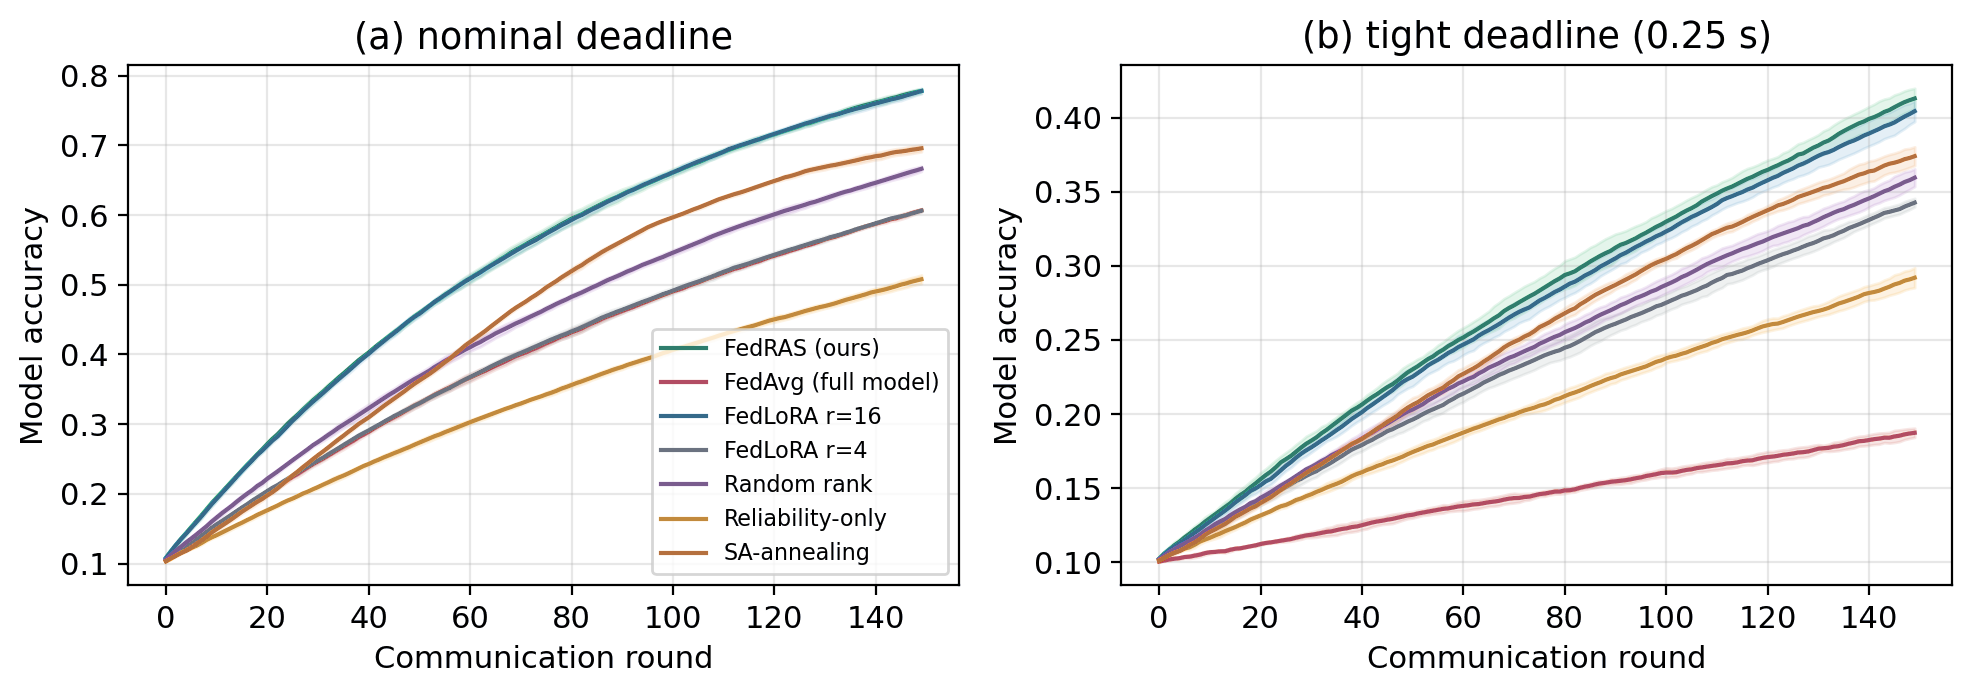
\includegraphics[width=0.8\columnwidth]{recolored_figures/sim_accuracy.png}
\caption{Scheduler simulation accuracy trajectories (mean$\pm$std, five seeds). Under the nominal deadline (left) FedRAS matches fixed rank 16. Under the 0.25\,s deadline (right) FedRAS downshifting separates from fixed rank 16 and outperforms random and full updates.}
\label{fig:sim}
\end{figure}

\begin{figure}[H]
\centering
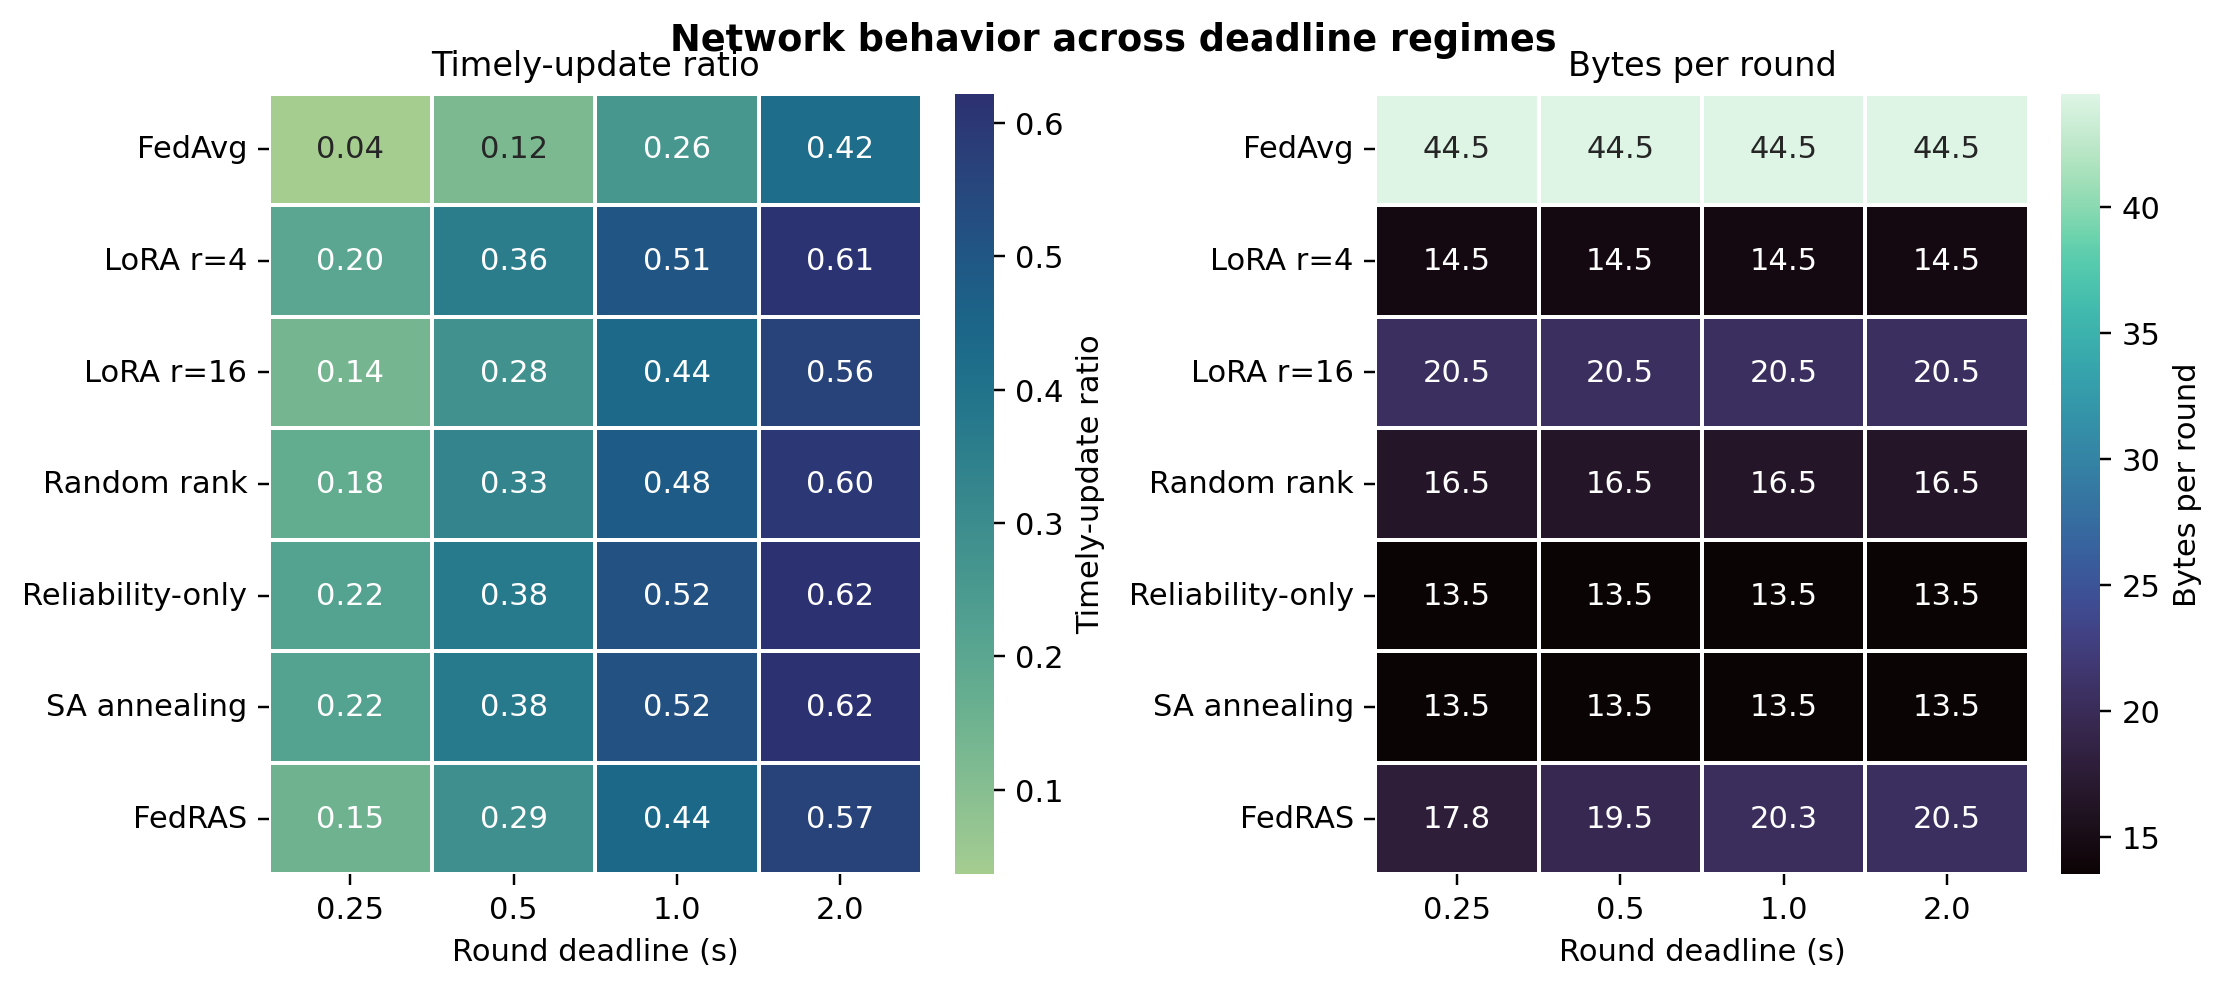
\includegraphics[width=0.8\columnwidth]{recolored_figures/sim_deadline_advanced.png}
\caption{Heatmaps of timely delivery ratio and bytes per round across deadline regimes in the 500-client simulator. Values are means over five seeds.}
\label{fig:simdl}
\end{figure}

Fig.~\ref{fig:sim} shows the nominal and 0.25\,s trajectories, and Fig.~\ref{fig:simdl} shows the network-side view. Full-parameter updates lose 86\% of their timely deliveries as the deadline tightens from the nominal deadline to 0.25\,s at a constant $2.2\times$ byte cost. The annealed schedule buys timely delivery by settling at rank 2, and FedRAS has comparable proxy accuracy and timely delivery to fixed rank 16 at 14\% fewer bytes.

\begin{table}[H]
\centering
\caption{Solver study with 500 clients, $K{=}25$, and 30 instances per cell. The table reports heuristic loss relative to the grid-based DP and DP runtime.}
\label{tab:dp}
\resizebox{\columnwidth}{!}{%
\begin{tabular}{cc ccc c}
\toprule
Deadline (s) & Budget (MB) & Greedy val/byte & Greedy value & Fixed $r{=}16$ & DP time (ms)\\
\midrule
1.0  & 300 & 0.0\% & 0.0\% & 0.0\% & 836\\
1.0  & 40  & 0.0\% & 0.0\% & 0.0\% & 92\\
1.0  & 12  & 6.1\% & 6.1\% & 6.1\% & 33\\
0.5  & 300 & 0.7\% & 0.0\% & 0.0\% & 833\\
0.5  & 40  & 0.8\% & 0.0\% & 0.0\% & 92\\
0.5  & 12  & 5.6\% & 6.0\% & 6.0\% & 33\\
0.25 & 300 & \textbf{9.7\%} & 0.0\% & 0.0\% & 830\\
0.25 & 40  & \textbf{10.0\%} & 0.0\% & 0.0\% & 92\\
0.25 & 12  & 4.5\% & 5.8\% & 5.8\% & 33\\
\bottomrule
\end{tabular}%
}
\end{table}

\subsection{Solver optimality and runtime}
\label{sec:dp_study}
Table~\ref{tab:dp} reports the scheduling study. When the byte budget is slack, greedy heuristics are near-optimal and the choice of scheduler matters little. The interesting regimes are the binding ones. When the budget binds at 12\,MB, value-per-byte greedy loses 4.5 to 6.1\% of the expected useful updates, and under a tight deadline it loses up to 10\% even when the budget is slack, with 9.7\% at 300\,MB and 10.0\% at 40\,MB, because per-byte ordering misprices delivery risk. The DP reaches the optimum of the discretized single-round estimated problem in every cell. Its runtime is 33 to 836\,ms for 500 clients depending on the budget-grid size, which the 0.05\,MB grid dominates, and it scales linearly to 1000 clients, as Fig.~\ref{fig:dp} shows. This is compatible with per-round scheduling at minute-scale FL rounds, and the grid step offers a tuning knob.

\begin{figure}[H]
\centering
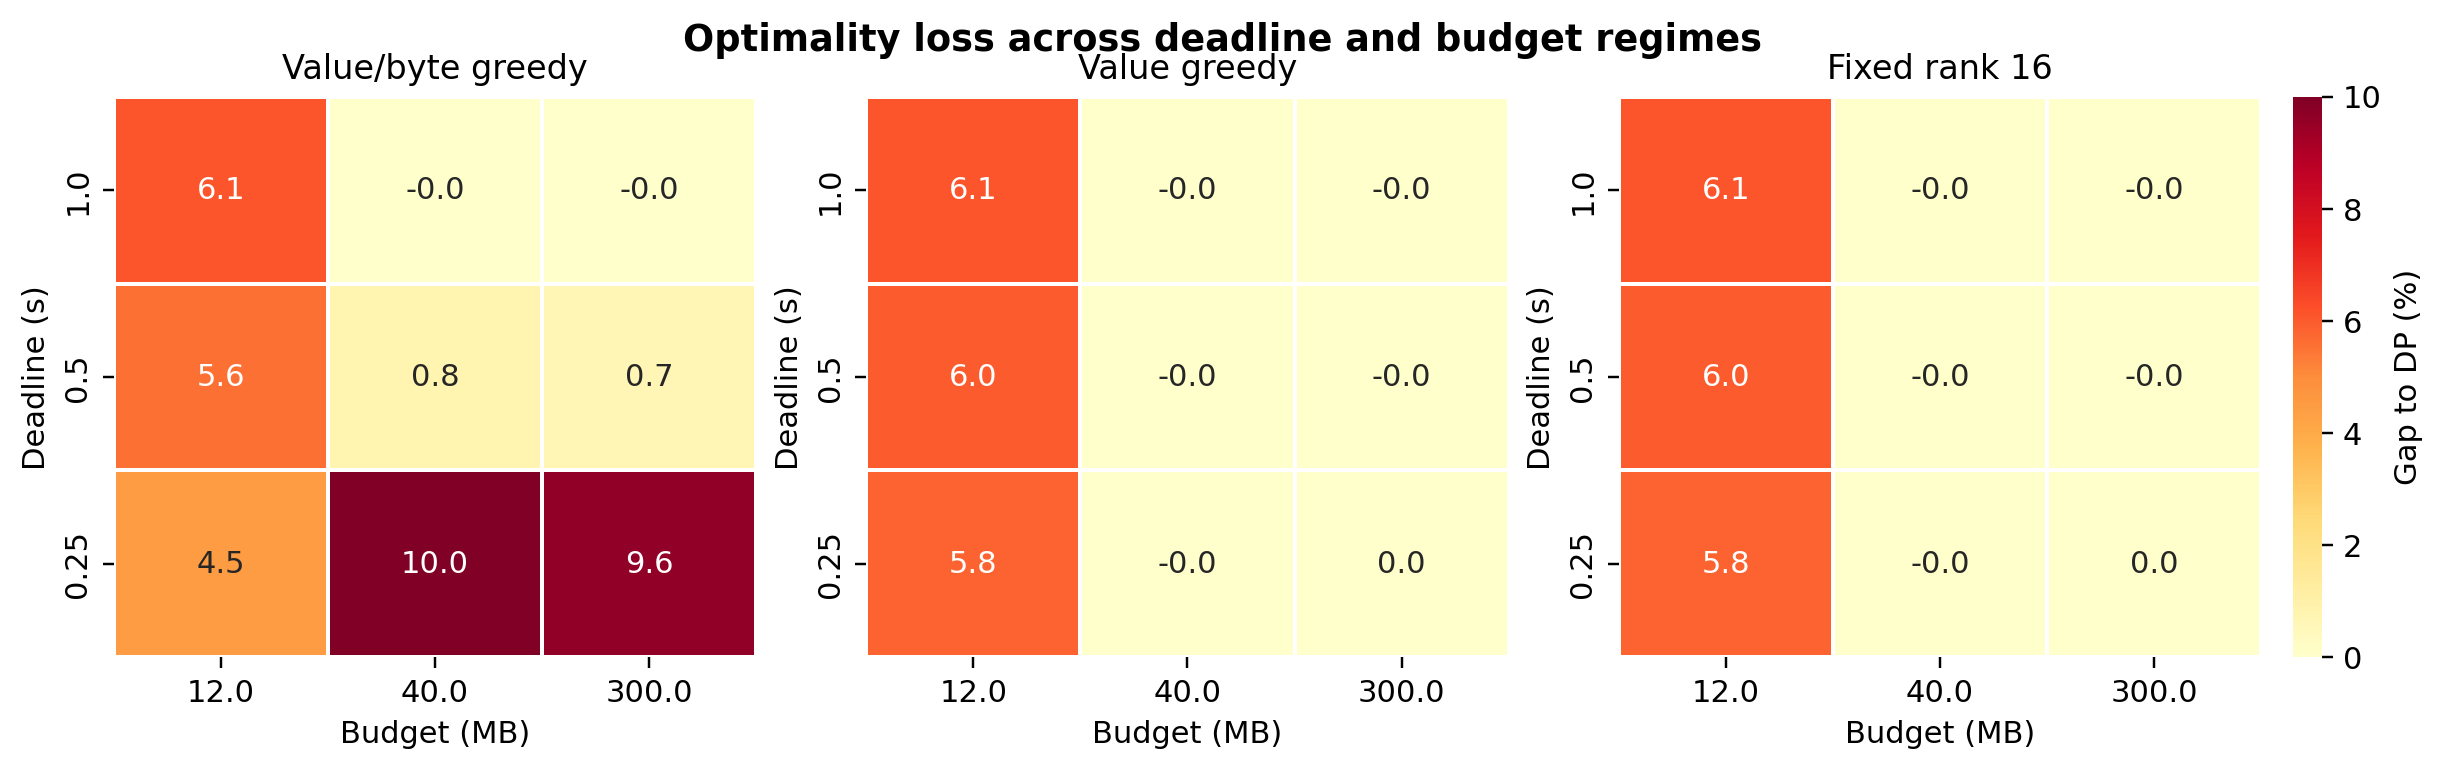
\includegraphics[width=0.8\columnwidth]{recolored_figures/dp_study_advanced.png}
\caption{Solver study. The heatmaps show objective loss relative to the DP solution across deadline and budget cells. The runtime curve shows scaling with client population.}
\label{fig:dp}
\end{figure}

A dedicated grid sweep with steps from 0.2 to 0.01\,MB and 30 instances per cell compares each step against a 0.01\,MB reference. When the budget is slack, the objective is step-insensitive, with 0\% deviation at every step. In the binding 12\,MB regime, the default 0.05\,MB step shifts the objective by at most 3.3\% across instances and deadlines, and a 0.025\,MB step bounds the deviation to 1.3\% at $1.7\times$ the runtime, that is, 27 to 45\,ms per round at 500 clients. The grid exactness claim of Section~\ref{sec:solver} therefore applies to a grid whose quantization error is bounded, measured, and adjustable at a known runtime cost. The fair-cohort variant used by the trainer, uniform sampling plus per-client argmax, reaches 27 to 55\% of the unconstrained DP objective. This is the price of population-fair participation rather than a defect of the FedRAS rank rule, and it delimits when full grid scheduling is worth its coordination cost.

\begin{figure}[H]
\centering
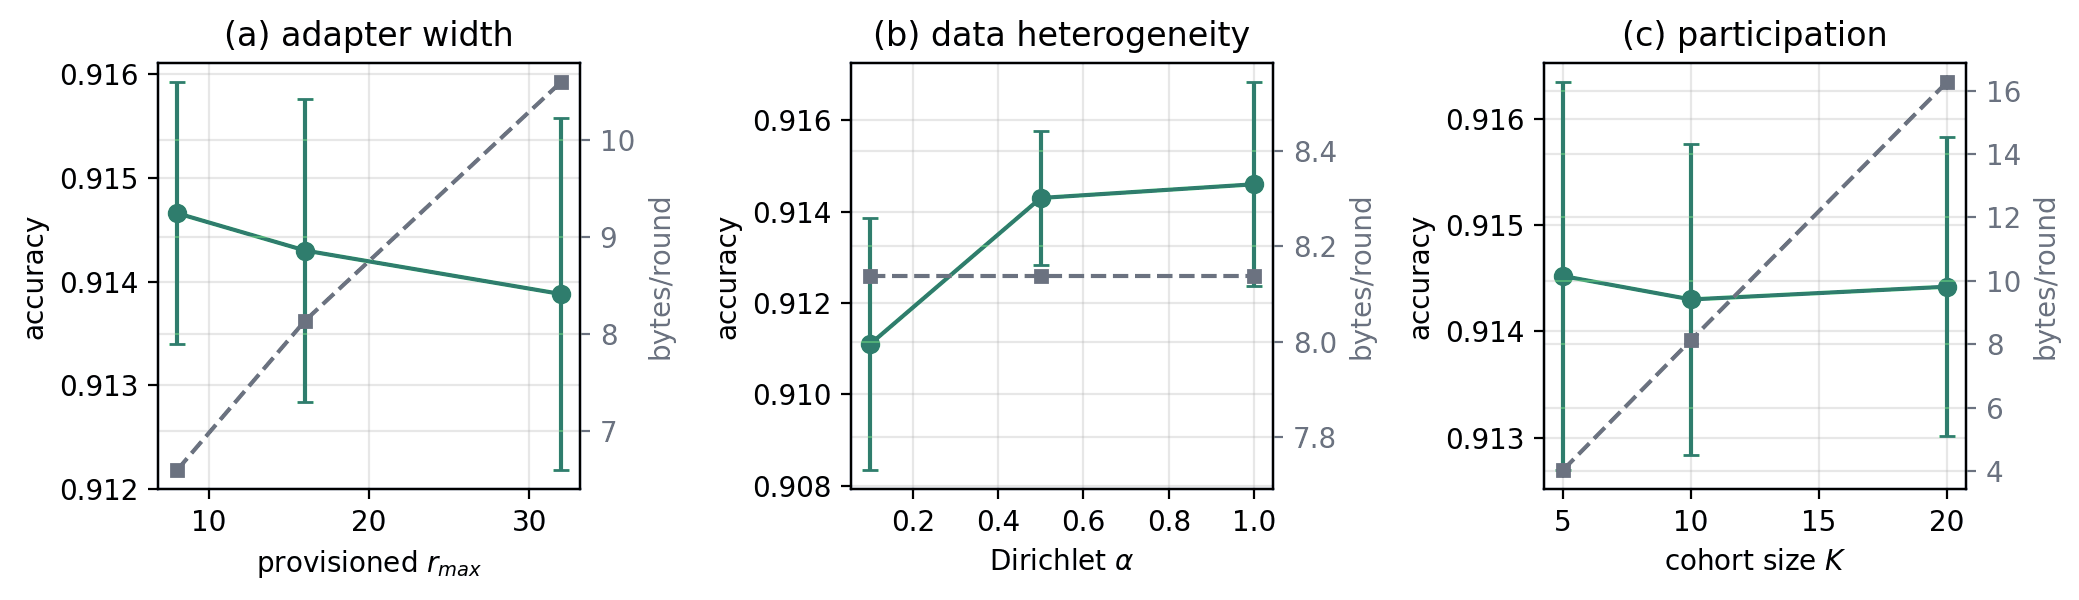
\includegraphics[width=0.98\columnwidth]{recolored_figures/sensitivity.png}
\caption{Sensitivity of the trainer to provisioned adapter width, label heterogeneity, and cohort size on CIFAR-10 with FedRAS. Results use five seeds and bars show $\pm$1\,std. Accuracy is flat in $r_{\max}$ and $K$ across the tested ranges; their effect is on bytes and delivered updates.}
\label{fig:sens}
\end{figure}

\subsection{Sensitivity analysis}
Fig.~\ref{fig:sens} varies the provisioned adapter width, the label heterogeneity, and the cohort size of the trainer on CIFAR-10 with five seeds. Widening the adapter from $r_{\max}=8$ to 32 leaves accuracy flat, while bytes rise from 6.6 to 10.6 and delivered updates fall from 4.8 to 3.9 per round. The provisioned width is therefore a network-facing decision rather than an accuracy control. Data heterogeneity from $\alpha=0.1$ to 1.0 moves accuracy from 0.911 to 0.915 at constant network cost, consistent with the parity claim across partitions. Cohort size $K$ from 5 to 20 leaves accuracy flat, while delivered updates grow from 2.3 to 8.6 per round at linearly scaled bytes. At the 0.25\,s deadline, the same growth is throttled by delivery, as the stress results above show. Per-decision scheduling cost is negligible in all settings. The per-client rank rule of the trainer costs 105\,$\mu$s per client--rank decision, about 1\,ms per round, against 33 to 836\,ms for the full grid-scheduling DP of Section~\ref{sec:dp_study}.

\textbf{Robustness to model error.} Two further simulation studies probe how much the scheduler depends on its own estimates. Injecting multiplicative lognormal noise with $\sigma=0.2$ into the predicted $\hat P_{\rm on}$ degrades the achieved objective by at most 5.1\% on average and 9.4\% in the worst instance, and only in the tightest deadline and budget cell. The slack regimes stay below 1\%. Mis-prediction therefore costs optimality smoothly rather than catastrophically, and the observed delivery outcomes of Algorithm~\ref{alg:scheduler} are exactly the signal a calibrated predictor would re-fit.

Replacing the square-root capacity form $G(r)$ with linear or logarithmic alternatives changes admission decisions by at most 0.5\% and the objective by at most 1.4\%. The value of the scheduler thus comes from coupling capacity with delivery risk, not from the specific saturating shape. The sublinear shape itself has an empirical anchor in the trainer, where the mean delivered update norm grows from rank 4 to rank 16 by $1.57\times$, which shows the diminishing returns the square-root model assumes and stays clearly below the $4\times$ linear scaling.

\begin{figure}[H]
\centering
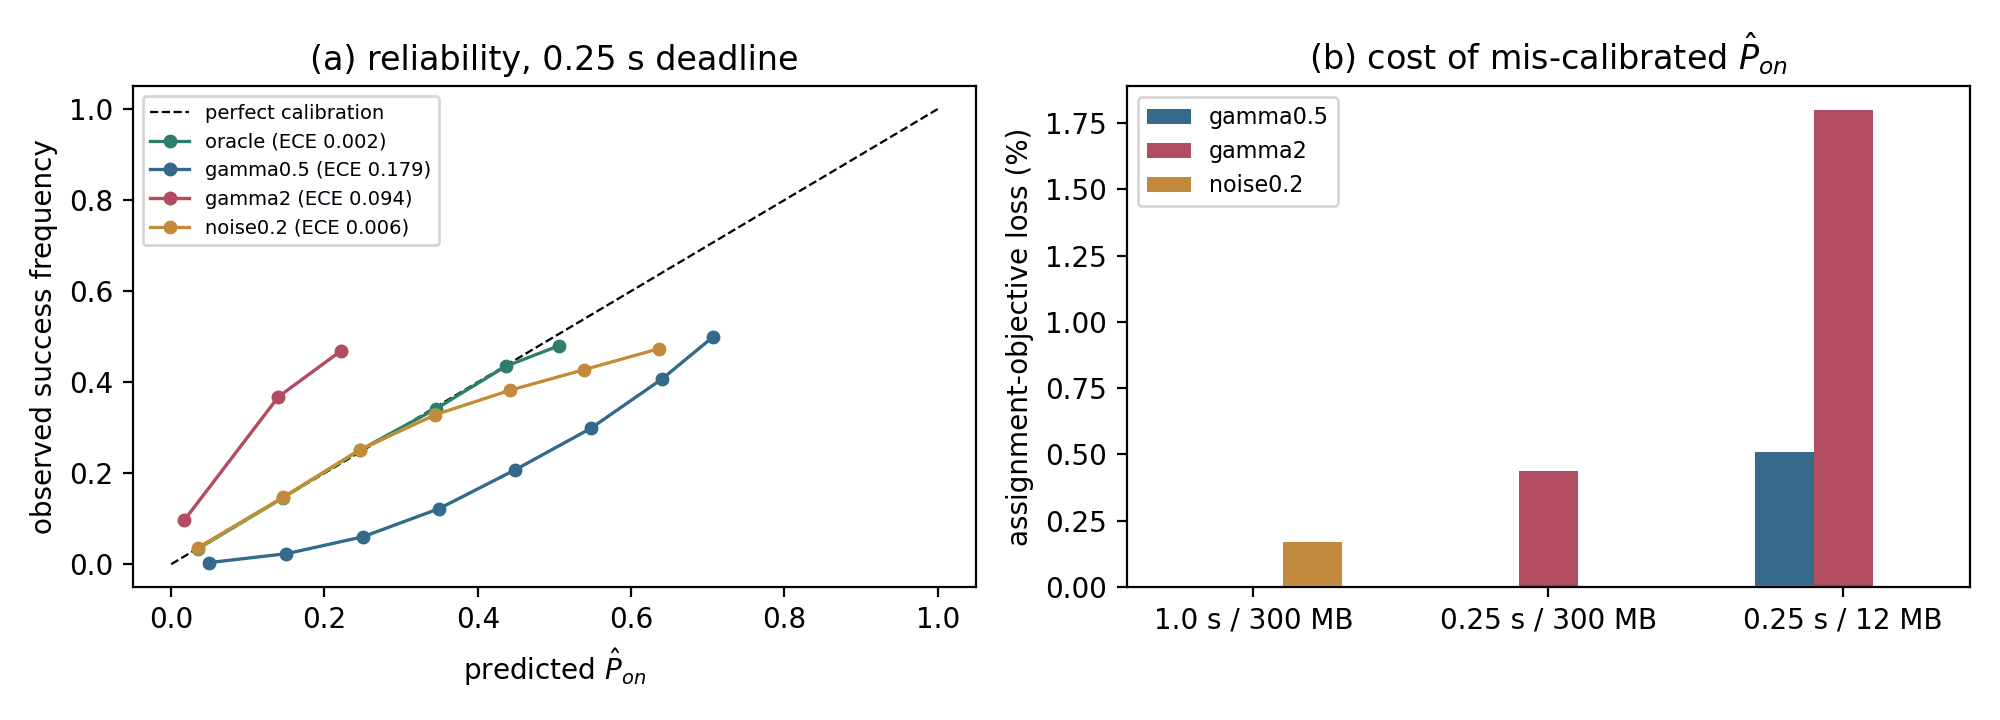
\includegraphics[width=0.8\columnwidth]{recolored_figures/fig_calibration.png}
\caption{Delivery-predictor calibration study (500 clients, 150 round-instances per cell). The left panel shows reliability at the 0.25\,s deadline. With oracle link state the hazard-form predictor is calibrated by construction, while the power-distorted ($\gamma$) and noisy variants are measurably miscalibrated. The right panel shows the assignment-objective loss of optimizing against the distorted predictor, evaluated under true probabilities, at most 1.8\% and only in the tightest cell.}
\label{fig:calib}
\end{figure}

\textbf{Calibration of the delivery predictor.} Calibration itself is measurable, and its scheduling cost is bounded, as Fig.~\ref{fig:calib} shows. On the link model of Section~\ref{sec:model}, the deployed predictor with oracle link state is calibrated by construction, with an expected calibration error of 0.002 to 0.004. Deliberately mis-calibrated variants $\hat P^{\gamma}$ with $\gamma$ of 0.5 and 2 reach an error up to 0.21, and multiplicative state noise with $\sigma=0.2$ up to 0.035. The resulting assignment-objective loss, however, stays at most 1.8\% and is confined to the tightest deadline and budget cell, with at most 0.5\% elsewhere. Even sizeable miscalibration therefore leaves the rank ordering largely intact, and the observed outcomes expose it for per-client recalibration. Calibration on measured traces remains open and is taken up in Section~\ref{sec:discussion}.

\subsection{Summary of findings}
\label{sec:summary}
Across both tiers, rank choice does not measurably change accuracy for the frozen backbone and 40-round horizon. The main differences are therefore on the network side. Full-parameter updates cost $2.2$ to $3.1\times$ the bytes, and they lose 54\% of their timely deliveries at 0.5\,s, 86\% at 0.25\,s, and 86\% in the simulation as deadlines tighten.

FedRAS behaves as designed, using high ranks on healthy links and downshifting under pressure. It saves 14\% of bytes while showing comparable accuracy and timely delivery to fixed rank 16 under stress. In the trainer, the full grid-scheduling arm with the same cap and an 8.2\,MB budget raises the timely delivery ratio from 0.42 to 0.56 at unchanged accuracy over ten seeds ($p=0.002$). Grid scheduling remains affordable, with sub-second per-round solving at 500 clients and its largest gains in binding-budget and tight-deadline regimes.

The statistical evidence rests on a ten-seed replication of the two headline trainer regimes, over seeds 0 to 9 with common random numbers within each seed. Versus fixed $r{=}16$ under the 0.25\,s deadline, FedRAS saves 14.5\% of bytes at the seed mean, with a bootstrap 95\% confidence interval from 12.4\% to 18.6\%, a two-sided Wilcoxon $p$ of 0.002, and a matched-pairs rank-biserial of magnitude 1.0. It delivers a higher timely delivery ratio in ten of ten seed pairs at $p=0.016$, while the accuracy difference is insignificant at $p=0.40$, and at $p=0.30$ under the nominal deadline.

Versus full-parameter updates the network-side differences are extreme, with 54\% and 61\% fewer bytes at the nominal and stress deadlines at $p=0.002$. The three external baselines replicate at ten seeds with accuracy parity and unchanged network-side structure. With five seeds alone, none of these tests could fall below $p=0.0625$. The statistical tests support the stated network-side comparisons. They concern network-side savings and accuracy parity. They do not establish accuracy dominance.

\section{Discussion and limitations}
\label{sec:discussion}
\textbf{Scope of claims.} The trainer demonstrates parity and not rank-dependent accuracy gains. With a strong frozen backbone and 40 adaptation rounds, transmitted rank does not measurably change test accuracy. Claims that low rank limits adaptation quality would require longer horizons, weaker backbones, or distribution-shifted clients. The simulator capacity model is a scheduling abstraction, and its accuracy is a bounded scheduling proxy rather than a measured dataset accuracy.

\textbf{Backbone pretraining.} The centralized pretraining stage is a documented premise inherited from parameter-efficient FL practice; the federated phase adapts but does not train the backbone. Where no server-side corpus exists, self-supervised or public-data pretraining would be needed, and the parity result should be re-verified.

\textbf{Estimator assumptions.} The hazard-form delivery model \eqref{eq:hazard} assumes the closed-form exponential realization. Production deployments should calibrate $P_{\rm on}$ per client from observed outcomes, for example with isotonic or Platt scaling monitored by a Brier score, and the scheduler treats the predictor as a plug-in.

\textbf{Myopia.} The DP is exact for the estimated per-round problem, not for the multi-round stochastic control problem induced by budget carry-over and mobility correlation; a horizon-aware policy could shift admissions across rounds and is a natural extension.

\textbf{Security.} This work schedules communication and does not propose protection, so we make no privacy claim. Frozen-factor training incidentally reduces the dimensionality of transmitted gradients, which shrinks the gradient-inversion surface. Formal statements require differential-privacy accounting or secure aggregation, which compose orthogonally with rank scheduling \cite{bonawitz2017secureagg,wei2023pfl_dp}.

A further observation from the stress matrix is that under extreme heterogeneity of $\alpha{=}0.1$, higher ranks lose a small amount of accuracy relative to rank 4, consistent with capacity-amplified client drift. The capacity term $G(r)$ could be conditioned on measured heterogeneity to capture this effect, which we leave as future work.

\textbf{Generality.} The trainer validates adapters on convolutional and linear layers of a CNN at $r_{\max}{=}16$ with 20--1000 clients and synthetic link traces. Extension to transformer backbones, measured rather than synthetic links, and larger rank sets may change the payload slope, capacity curve, and empirical conclusions. The formulation can be tested in those settings. The study does not measure energy, system overhead beyond scheduler runtime, or client fairness and therefore makes no claim about those properties.

\section{Conclusion}
\label{sec:conclusion}
This paper reframed Federated LoRA over mobile edge networks as a deadline-aware client--rank scheduling problem in which the LoRA rank is a network-visible resource. We derived a rank-dependent delivery model with an explicit MB-to-Mbit hazard, formulated the per-round assignment as a multiple-choice knapsack under budget and participation caps, solved the grid-discretized assignment with a pseudo-polynomial dynamic program, and stabilized heterogeneous-rank aggregation with frozen-factor rank-masked averaging.

Experiments with a real federated LoRA trainer and a 500-client scheduling simulator show that FedRAS preserves backbone accuracy, saves 14\% of update bytes while showing comparable accuracy and timely delivery to fixed rank 16 under five-seed deadline stress, and exposes the collapse of full-parameter updates, which cost $2.2\times$ the bytes and deliver only 4\% of updates on time at a 0.25\,s deadline. The grid-based scheduler recovers up to 10\% expected useful updates over greedy heuristics in binding regimes at sub-second cost. Future work includes horizon-aware stochastic scheduling, calibrated per-client delivery predictors, protection mechanisms composed with rank scheduling, and validation on measured mobile traces and transformer backbones.

\section*{Declaration of competing interest}
The authors declare that they have no known competing financial interests or personal relationships that could have appeared to influence the work reported in this paper.

\section*{Acknowledgements}
The authors thank the members of the Information Engineering University research group for many useful discussions and for hands-on assistance with the experimental implementation.

\section*{Funding}
This research did not receive any specific grant from funding agencies in the public, commercial, or not-for-profit sectors.

\section*{CRediT authorship contribution statement}
\textbf{Wenyu Ma:} Methodology, Software, Validation, Investigation, Writing -- original draft.
\textbf{Tao Hu:} Conceptualization, Formal analysis, Supervision, Writing -- review and editing.
\textbf{Xinlei Liu:} Data curation, Investigation, Visualization.
All authors approved the submitted version and accept responsibility for the work.

\section*{Data availability}
The reproducibility package accompanying this submission contains the complete source code (trainer, simulator, solver, and analysis scripts), per-run configuration files, per-seed result tables, and the raw training logs supporting every table and figure in this study; a permanent repository DOI will be supplied at publication.

\section*{Declaration of generative AI and AI-assisted technologies in the manuscript preparation process}
During the preparation of this work the authors used AI-assisted tools for language editing and formatting support. The authors reviewed and edited all generated material and take full responsibility for the content of the published article.

\bibliographystyle{elsarticle-num}
\bibliography{references}
\end{document}












